\part{Core}
\label{part:core}

In the core part of the thesis we present o-ur main contribution, consisting of research and applications towards better interlinking of information on the Semantic Desktop. We introduce interlinking of personal notes with the semantic note-taking tool SemNotes, then we present a method for connecting Semantic Desktop data to the Web of Data, followed by the description of a use case and system for semantic publishing which incorporates and builds on the two previous chapters. Each of the chapters is based on previously published works.

We start from the premise of the Semantic Desktop --- it provides the framework we need for building our network of linked personal information. The order of the chapters follows the logical order of interconnecting Semantic Desktop information. 

We start at a local level in Chapter \ref{ch:semnotes}, by describing ways of creating new semantic data within the desktop, integrating it with the existing information from the desktop, and making it accessible across application borders. In this context, we present the challenges we found and our solutions to semantic application development on the Semantic Desktop.

Since the personal information we use is no longer restricted to the desktop, it has become important to expand the network of personal linked data beyond the desktop, into the Web of Data. Making use of the large amount of data available online in linked form, in Chapter \ref{ch:sdwod} we describe a method for bridging the gap between the two linked data networks --- the Semantic Desktop and the Web of Data. 

In Chapter \ref{ch:semblogging} we merge the interlinking of new notes with existing semantic desktop data from Chapter \ref{ch:semnotes} with the interlinking of the same data with Semantic Web from Chapter \ref{ch:sdwod}, for the purpose of semantic publishing. The solution we present is not limited to the use case of semantic blogging, but it is valid also for e-health use cases like patient records and doctor notes, or for the enterprise domain, for reporting or collaboration. 

In the last chapter of the section, Chapter \ref{ch:mischelperapps}, we describe several other proof of concept applications we developed with the same goal of enabling and supporting better interlinking of personal data on the desktop and beyond. 

The work builds on top of the Nepomuk-KDE branch of the NEPOMUK Social Semantic Desktop, described in detail in Section \ref{sub:nepomuk} and it reuses the ontologies defined within the NEPOMUK project. Using the libraries and vocabularies in an application has led, as a collateral result, to improvements and changes in both.


\chapter
{Creating and Interlinking Semantic Data on the Desktop with SemNotes}
\label{ch:semnotes}

\begin{flushright}
 \textit{Based on ``The Semantic Desktop at Work: Interlinking Notes'' \cite{Dragan2011a}\\published at the 7th International Conference on Semantic Systems (I-SEMANTICS~2011)}
\end{flushright}

The Semantic Desktop has been proposed as a solution to the ever growing problem of information overload on our computers. It provides the foundations necessary to integrate and manage personal information. However, the challenge of designing and realising semantic applications that use this infrastructure still remains. 
In this chapter, we present SemNotes\footnote{\url{http://smile.deri.ie/projects/semn}}, a semantic note-taking tool for the Nepomuk-KDE Semantic Desktop, as a tool for creating new semantic information on the desktop and integrating it seamlessly in the existing network of linked desktop data.
SemNotes provides a real-world, functional use case for fully exploiting the capabilities of the Semantic Desktop: interlinking, organisation and management of personal information, improved search and browsing. 
Furthermore, it represents our solution to a set of identified generic challenges for applications on the Semantic Desktop, as described by the first research question in Section \ref{sub:question}.
We describe a task-based user evaluation comparing SemNotes with a conventional note-taking tool. The results show that complex searches on interlinked information created with SemNotes are significantly faster, with little or no extra effort required from the users. 

\section{Introduction}
\label{sec:semnotesintro}

The Semantic Desktop provides a framework for creating applications and tools that simplify the daunting tasks of managing personal information accumulated on the desktop. 
The information overload problem, combined with the disconnection of data caused by application silos, is solved by the use of Semantic Web standards for storing and interlinking the desktop information. 
Data which before was stored separately by different applications can be now explicitly connected. The result is a network of interlinked personal information, which can be browsed by association, filtered and searched in a unified way. 

The Semantic Desktop overcomes the limitations of conventional desktops, where information is kept in different formats and application repositories, by using common vocabularies to describe the data, and a desktop-central place to store it, in a standardised format, accessible to all applications.

Indeed, the Semantic Desktop makes the information load manageable. However, new challenges emerge: one such new issue is how to design and realise semantic applications that use the infrastructure provided by the Semantic Desktop. We address this problem by dividing it into smaller, simpler challenges and providing solutions for each of them. To illustrate the solutions, we describe the design of a semantic note-taking application for the Nepomuk-KDE Semantic Desktop, called SemNotes. We use note-taking as an example because it is a desktop activity that is not limited to a specific domain, since the notes can widely vary in topic. It is also a common activity that plays an important role in Personal Information Management and that we believe would benefit from the use of semantic technologies.

\subsection{Challenges}
\label{sub:appchallenges}

In Section \ref{sub:question} we broke down the first research question \textbf{Q 1.}: \emph{How to build semantic applications and tools for the Semantic Desktop as to provide the best experience for the users, while creating reusable semantic data?}, into several sub-questions.
These are the challenges we found in designing new semantic applications for the Semantic Desktop:

\begin{description}
 \item[Q 1.1.] \emph{How to create semantic data that is correct, and maximises the reuse of existing Semantic Desktop data through interlinking?}\\
Applications should be aware of the data that is available on the desktop, from other applications. The data they produce is also accessible to other applications, and this should also be taken into account, because it raises the dual challenge of making sure that the data is represented correctly so that other applications can use it if they choose, as well as making the most of existing information through reuse and link creation. How to interlink information items is the most important challenge for adhering to the Semantic Desktop requirements of creating and maintaining a network of linked desktop data. It refers in the first place to the new information coming into the desktop through the application, and how to integrate it with the linked information that exists on the desktop. But it also covers the situation when the only new information created is in fact a new link between existing entities. 
Existing desktop data is heterogeneous. The reasons for this include the fact that different parts of it are created by different applications, with different functionalities and needs. So, although represented in a standardised way, the data is not always consistent, up-to-date or even correct. Furthermore, the data is also heterogeneous in terms of form: there are new types of information available to be integrated (i.e. tags, relations). Best practices advise the reuse of as much of the existing information as possible, because through reuse, the interlinking becomes deeper and richer. However, the possibility of reusing vast amounts of existing data raises other challenges, in selecting the right amount of necessary information for maximum benefit for the users, while not overloading them. The selection is complemented by the way the information is shown.
 \item[Q 1.2.] \emph{How to design the human-computer interaction in an application for the Semantic Desktop?}\\
This question relates to designing interfaces which support the existing workflow of the user, while integrating the additional semantic information in a useful way. A balance must be found between too much information, so that it interferes with the user doing tasks, and too little, or not enough to make a difference. The question also refers to more than just displaying the information in an interface --- allowing users to interlink information items easily, and generally aiding the creation of new semantic data is also a challenge for application development. Extra difficulty is added by the variety of interlinked information available on the desktop, combined with the reduced control of developers over what resources are linked from other tools.
 \item[Q 1.3.] \emph{How to correctly evaluate a semantic application?}\\
A challenge related to evaluation is the lack of a standardised dataset to use, due to the highly personal data required. Even if such a dataset existed, due to the fact that the applications on the Semantic Desktop are mainly related to personal information, it is difficult for participants to use the data provided, as they are not familiar with it. Evaluating PIM tools has been shown to yield best results when the test users are asked to perform their own tasks in their own set-up rather than attempting to simulate it with artificial tasks and artificial data. The reduced number of semantic application in each area makes it difficult to evaluate a new tool against an existing established one, thus the best candidates for a comparative evaluation are conventional (i.e. not semantic) applications with similar functionality. While possibly re-demonstrating that indeed linked data is more useful, comparing a semantic and non-semantic application requires well thought metrics, as the semantic features that need 
evaluating have no direct counterparts against which to evaluate them. For task based evaluations, it is difficult to find a common set of tasks that both applications can perform. A solution is to choose general, high level tasks, but that influences the granularity of the results.
\end{description}


\section{Tackling the Challenges: The Design of SemNotes}
\label{sec:semnotesdesign}

We use our note-taking application, SemNotes, to describe the general principles we used for designing an application for the Semantic Desktop. Note-taking is a good general use case for the Semantic Desktop because the information contained in notes is not restricted to a specific domain. Personal notes are naturally connected to the user's context, and can thus be meaningfully interconnected with much of the existing network of personal data on the desktop.

We divided the design into specialised modules. Each module handles a set of related tasks. We describe the modules as they would be for a general semantic application, followed by a more specific description about the implementation of SemNotes in the next section.
 
\subsection{Data Representation} 

This module handles the vocabulary of the application: the \emph{data types} around which the application is centred, and the kind of \emph{metadata} that is needed for them. To enable other Semantic Desktop applications to understand the data produced, as well as for our application to understand data from the underlying Semantic Desktop, the best practice is to reuse existing desktop ontologies where possible. The basic data type handled by SemNotes is the note, represented by a short snippet of text containing personal information. 

\subsection{Data Management} 

This module manages the life-cycle of the semantic data that the application handles, by enabling the transition between the phases of the life-cycle. We adapted the Abstract Data Life-Cycle Model \cite{MoellerPhDThesis2009} to illustrate a comprehensive workflow for Semantic Desktop data, from its creation to its termination. Figure~\ref{fig:datalifecycle} shows the phases and transitions between them, focusing on the possible actions that the user can execute, and hence, that a semantic application could support.

\begin{figure}[htb]
 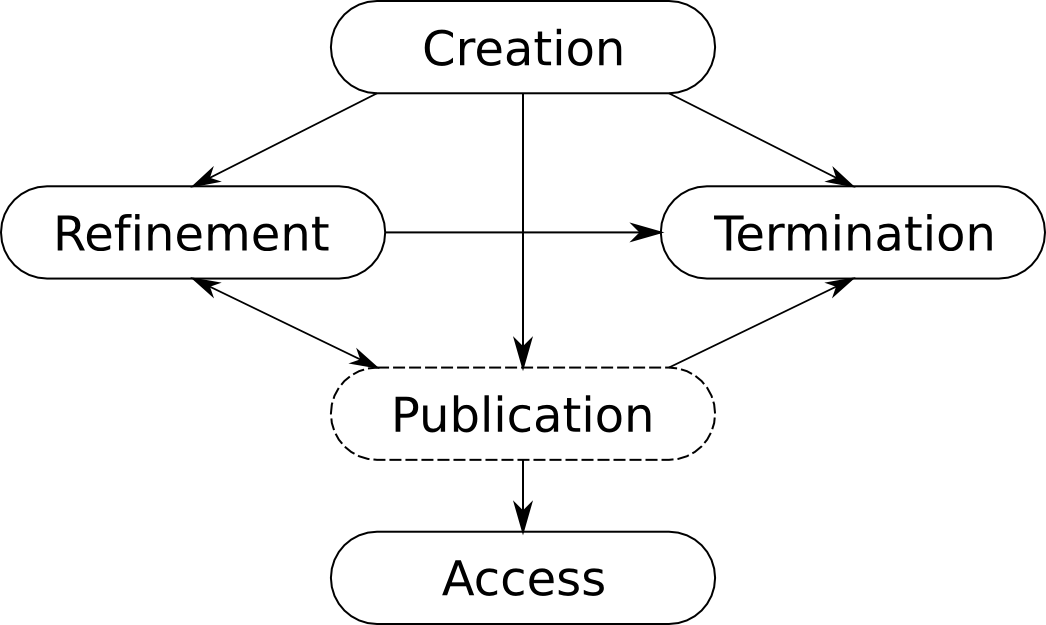
\includegraphics[width=0.7\linewidth]{chapters/core/img/lifecycle}
\caption{Semantic Desktop data life-cycle.}
\label{fig:datalifecycle}
\end{figure} 

\begin{description}
 \item[Creation.] Most often creation implies creating a new resource, of a given type. However, the import of existing data from other applications or formats (e.g. crawlers) is also included here.
 \item[Refinement.] This phase includes any activities that make changes to existing data. It also contains the creation and deletion of links between existing resources, although alternatively they can be included in the Creation or Termination phases, as links are data too. 
 \item[Access.] This phase is represented by accessing the data through either querying or browsing. Because we are discussing interlinked data, accessing a piece of semantic data implies recursively accessing the sub-graph of resources semantically related to it. How much of the sub-graph is traversed can vary, and further traversal by the user should be supported and encouraged. 
 \item[Termination.] In this phase the data is deleted from the system. As with the access phase, rules must be defined to determine how much of the dataset a deletion will affect---e.g. it might make sense to delete all the subtasks of a task when the parent is deleted, but not to delete the documents related to the task.
 \item[Publication.] This phase represents making the data accessible to users from outside the system. Also included here is exporting the data to other formats and applications. When handling semantic personal data, applications should ensure that sensitive data is well protected against unauthorised or accidental publication. 
\end{description}

Furthermore, this module handles where and how the data is stored. The Semantic Desktop provides the framework for storing semantic data, therefore it is best that the central desktop repository be used, when practical. This enables easier interlinking with the rest of the data. In the case of SemNotes, the notes and all the metadata about them are stored in the desktop repository. 

\subsection{Interlinking} 

The interlinking module is logically a sub-module of the Data management one, as it specifically manages a part of the refinement phase of the data life-cycle. However, because it is an important part of any semantic application, relating to the first two challenges listed in Section \ref{sub:appchallenges}, we describe it as a standalone module. The interlinking module effectively realises the goal of integrating the new semantic data into the pool of existing linked desktop data. The functionalities offered can vary from simple automatic linking of new resources to a specified context or to their author, to complex extraction and inference of new relations and resources.  This module provides the feature that sets SemNotes apart from other note-taking tools, the interlinking of the notes with the desktop resources mentioned in them. In our application, there are two sub-modules, that handle \begin{inparaenum}[(i)] \item entity recognition, and \item information extraction\end{inparaenum}, suggesting 
possible new connections to be created by the user.
 
\subsection{Visualisation} 

The visualisation module presents the data to the user in a simple, yet useful and versatile way. It addresses the third challenge listed above: designing the interface. Depending on the application, the visualisation can include \emph{aggregated} views on the data, and \emph{filters}. Faceted search \cite{Yee2003} has proven useful for semantic data, and it can be used to present the interlinked information to the user in a meaningful way. In SemNotes, the data that needs to be visualised is basically an enhanced version of a list of notes, with sorting and filtering. The module also provides the note editor. An important part of the module is displaying the recommendations for interlinking, a difficult task due to the heterogeneous nature of the information to be presented in a uniform, uncluttered way.

We describe how we tackled the last question --- the evaluation of the application --- in Section \ref{sec:semnotesevaluation}. 


\section{Implementation of SemNotes}
\label{sec:semnotesimplementation}

In the development of SemNotes, we tried to reuse as much as possible of the features provided by the host Semantic Desktop, Nepomuk-KDE\@. Using the existing functionality enabled better integration with the rest of the system, while reducing the effort required for the implementation. Nepomuk-KDE provides out of the box central RDF storage for the desktop, and an efficient means to access and query the data. 

We describe below the implementation of each of the modules introduced in the design section. 

\subsection{Data Representation} 
\label{sub:datarepresentation}

We describe the data created by SemNotes using a subset of the desktop ontologies described in Section \ref{sub:nepomuk} --- Personal Information Model (PIMO) and Nepomuk Annotation Ontology (NAO). 
Figure~\ref{fig:holiday} shows a basic note with metadata, and Listing \ref{lst:noterdf} contains the Turtle representation of the same example. 

The central unit of information handled by SemNotes is the note --- represented as an instance of \verb|pimo:Note|. 
The information stored for each note consists of: 
\begin{itemize}
 \item title --- \verb|nao:prefLabel|
 \item content --- \verb|nao:description|
 \item creation date --- \verb|nao:created|
 \item last modification date --- \verb|nao:lastModified|
 \item rating --- \verb|nao:numericRating|
 \item tags --- \verb|nao:hasTag|
 \item related desktop resources --- \verb|pimo:isRelated|
\end{itemize}

The Nepomuk ontologies make the distinction between resources representing native computer structures, which are described with the Nepomuk Information Element (NIE) ontology and resources representing concepts in the real world, which are described with the Personal Information Model (PIMO).

Before representing the PIMO concepts, most of the semantic data on the desktop is extracted from \verb|nie:DataObject|s and interpreted as \verb|nie:InformationElement|s. This is due to the fact that generally the information is still created by non-semantic applications, and to make it useful to the Semantic Desktop it has to be transformed, while keeping provenance information and feeding back into the applications that created it.

The extra step of extracting resources is not needed in the case of the information created directly for the Semantic Desktop by semantic applications. Thus, if no data is stored outside of the repository, no NIE resources are created. This is a characteristic of SemNotes and of other semantic applications for the Semantic Desktop.

The \verb|pimo:Note|s created with SemNotes can however be exported as text or HTML files, for backup or other purposes, thus associating a NIE resource to a note. This is the reverse of the usual process, and the change stems from working directly with the framework provided by the Semantic Desktop.

\begin{figure}[th]
 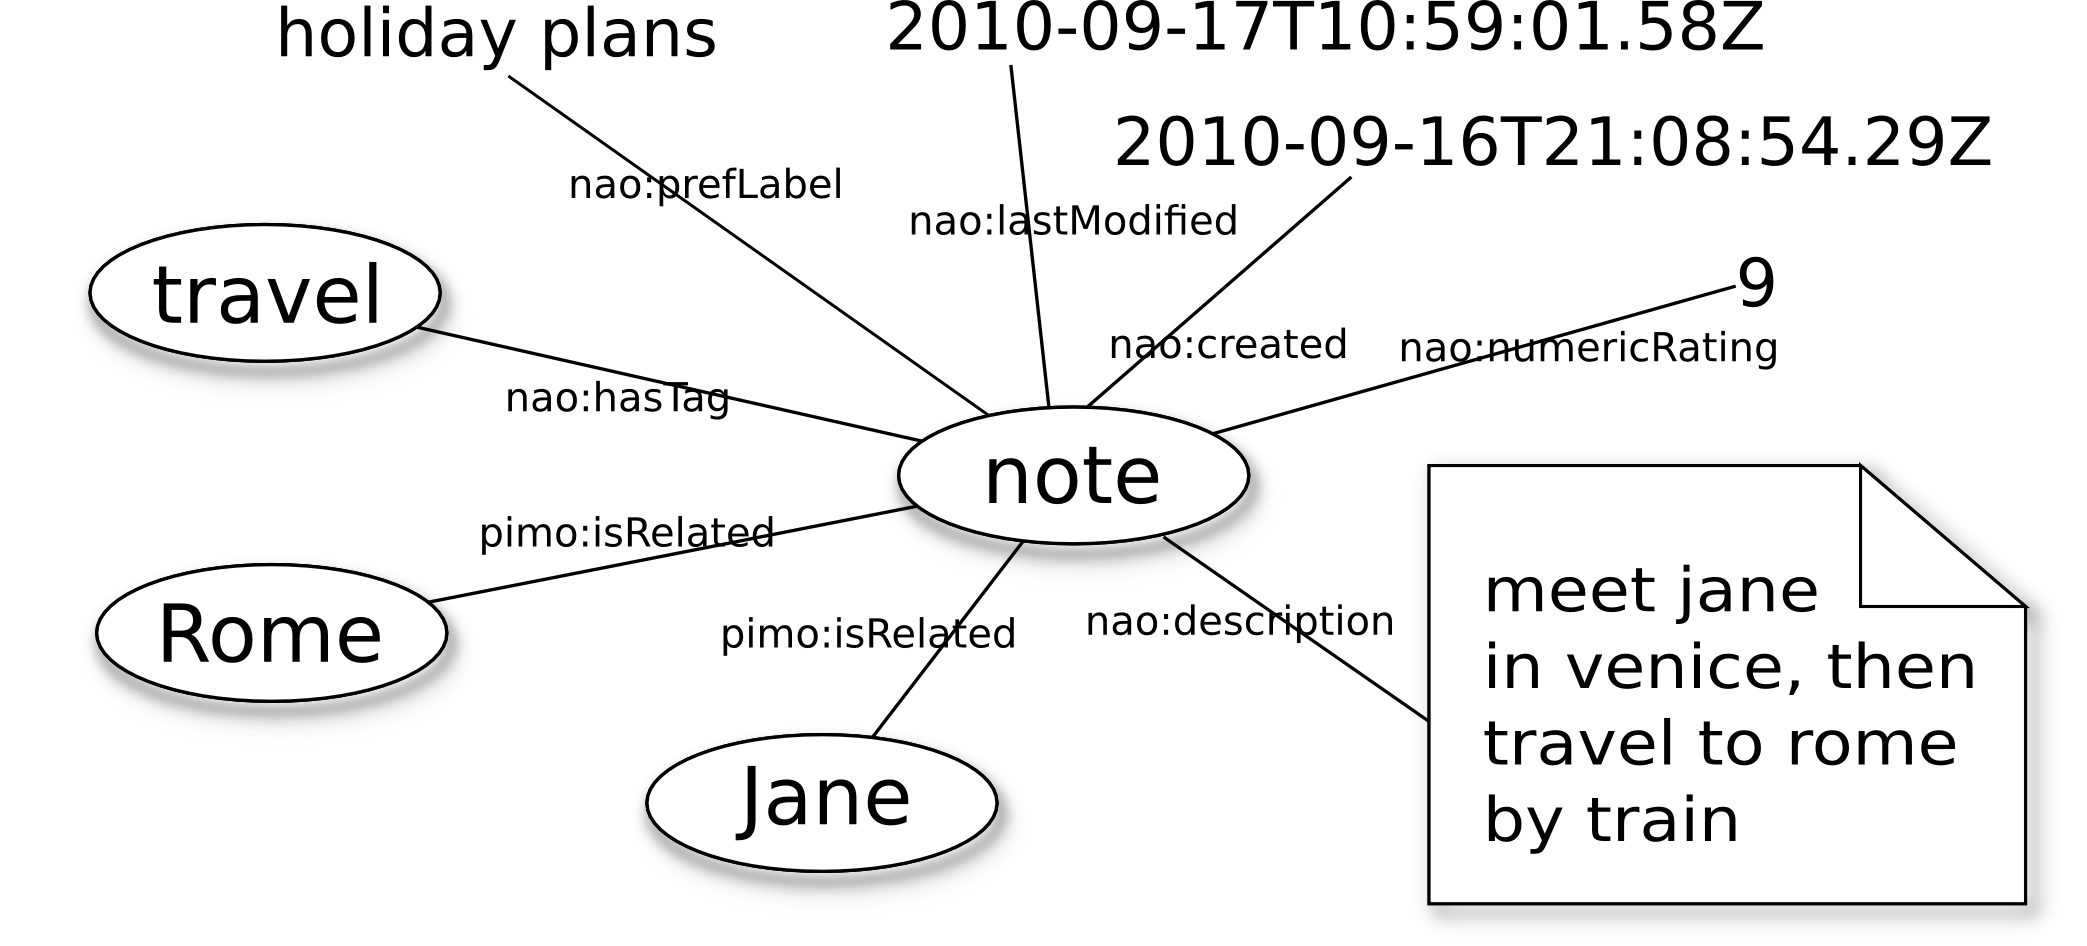
\includegraphics[width=0.9\linewidth]{chapters/core/img/note-properties}
\caption{Graph representation of the information about a note.}
\label{fig:holiday}
\end{figure} 

\subsubsection{Note metadata}

Tagging, rating and commenting are basic features provided out of the box by the Nepomuk-KDE system, for all types of resources. 
In SemNotes the only categorisation mechanism we use are tags, preferring simplicity over the more accurate mix of categories, topics and tags. The \verb|nao:hasTag| relation links the note to system-wide tag instances, thus enabling the reuse of tags throughout all applications, reducing duplication of classification work for the user. 

We later added support for rating to the interface, leaving the meaning of the rating open for the user to decide --- some possible examples include importance, urgency, quality of the content, or readiness for publication (in the case of a draft blog post as will be shown in Chapter \ref{ch:mischelperapps}).

Commenting on notes, although supported by the underlying system, because notes are resources, is not supported in the interface of SemNotes. We made this decision because the notes are themselves a type of comment, and we considered the feature redundant. 

\lstset{
	caption={RDF representation of a note.}, 
	label=lst:noterdf,
	language=turtle
}
\setlength\parindent{0in}
\begin{minipage}[t]{\linewidth}
\begin{lstlisting}
@prefix xsd: <http://www.w3.org/2001/XMLSchema#> .
@prefix pimo: <http://www.semanticdesktop.org/ontologies/2007/11/01/pimo#> .
@prefix nao: <http://www.semanticdesktop.org/ontologies/2007/08/15/nao#> .

<nepomuk:/res/thenoteuri> a pimo:Note ;
       nao:prefLabel "holiday plans"^^xsd:string ;
       nao:description "<html>...</html>"^^xsd:string ;
       nao:created "2010-09-16T21:08:54.29Z"^^xsd:dateTime ;
       nao:lastModified "2010-09-17T10:59:01.58Z"^^xsd:dateTime ;
       nao:numericRating "9"^^xsd:int ;
       nao:hasTag <nepomuk:/res/travel> ;
       pimo:isRelated <nepomuk:/res/Rome>, <nepomuk:/res/Jane> .
\end{lstlisting}
\end{minipage}
\setlength\parindent{0.21in}

\subsubsection{Note content}

Because notes are generally short \cite{Bernstein2008} we decided to store the note content in the RDF repository, as a property of the note (\verb|nao:description|). The value is the HTML string representing the content of the note, including formatting. This decision enables us to use the indexing and full text search feature provided by Nepomuk-KDE. 

Using the general property \verb|nao:description| to store the content of the notes, opens up the possibility of treating any semantic resource on the desktop as a note in SemNotes. This is equivalent to adding comments on each resource, but employing the functionalities provided by the application, including the analysis of the text to suggest relations. This enables serendipity --- discovering non-obvious connections between any desktop resources.

\subsubsection{Related resources}
 
As we discussed, the most important feature of SemNotes is the interlinking of notes with relevant resources from the desktop. The relations are stored using \verb|pimo:isRelated|. In the current revision of SemNotes, this is the only type of relation. This decision was based on the results of the long term study of Gnowsis usage \cite{Sauermann2008} which found that for PIM tasks it is enough to express that two things are related, and that the simpler properties are preferred by users over the more specific ones, regardless of the possible loss of meaning. However, we consider extending the range of possible relations in future versions. Having the information about the resources that are linked, specifically about the type of the resources, we can infer the possible relations to suggest, based also on knowledge from the desktop ontologies. 

Restricting the types of possible relations also keeps the interface simple, which was one of the design goals, and one of the biggest challenges we encountered, as we show in more detail in \ref{sub:semnotesvisualization}. We further explain the extraction and creation of relations in \ref{sub:interlinking}.

\subsection{Data Management}
\label{sub:datamanagement}

SemNotes supports all the phases of the note life-cycle.

When a new note is created, a new URI is generated for it, and the creation time is set. The rest of the properties are not set at creation time. As note data is added (i.e. the refinement phase), the metadata about the note and the content is updated. At each new update or annotation of the note, the last modification date is also updated. The notes can be found (i.e. the access phase) through full-text search, filtering by tags, related resources, and by creation date. Once the required note is found, it can be viewed in the editor. When a note is deleted, all metadata and relations about it are deleted as well, however, none of the tags and related resources are removed from the system, as they might originate from, or be used by other applications. The publication phase is also supported by SemNotes, as notes can be exported as HTML or text files, or even directly published online as blog posts \cite{Dragan2010a}.

As mentioned above, SemNotes uses the RDF repository provided by Nepomuk-KDE for all data storage. 

\subsection{Interlinking}
\label{sub:interlinking}
The interlinking of notes with related resources is the key feature of SemNotes. This feature realises the actual integration of the new information with the existing network of linked desktop data. Annotating the notes with related information captures the context of the note. Context is important for personal information management because it enables reminding and better (more precise, faster) search. Links between resources also support wayfinding \cite{Jones2008KFTFBook} and encourage exploratory browsing and serendipity.

The module uses entity recognition and string matching algorithms to detect and suggest possible related resources, but no link is created until the user selects the correct one. This mixed-initiative approach is a compromise between the precision of the links created and the amount of interference with the user's workflow.

The current implementation suggests annotations based on the knowledge about existing desktop resources, using entity matching techniques to identify the likely candidates. Certain types of resources are more likely to be related to notes (e.g. people, organisations, projects, events, tasks, other notes, locations). By default, SemNotes restricts the search for suggested resources to these types, but the user can easily modify the list. We do not include every resource on the desktop because of the large number of files that are indexed by the Semantic Desktop, which would clutter the suggestion list. For the resources of the given types, all textual properties are compared against the note text. This way, resources that do not explicitly have the search term in their label will show up in the suggestion list. An example is shown in Figure~\ref{fig:annotation}: for the word ``John'' other notes that mention him are suggested, even though his name is not present in the label.

\begin{figure}[tb]
 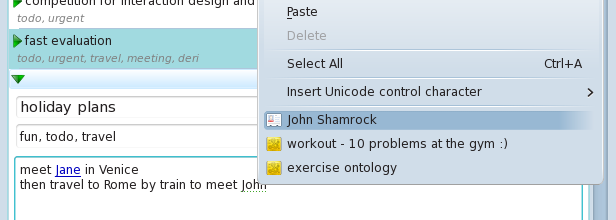
\includegraphics[width=\linewidth]{chapters/core/img/semnotes-screenshot-menu}
\caption{SemNotes annotation suggestion and link.}
\label{fig:annotation}
\end{figure} 

SemNotes does not currently offer suggestions based on online resources\footnote{Similar to \url{www.zemanta.com}.}, unless there is a desktop resource previously created for the relevant Web data (i.e. a bookmarked Web page becomes a desktop resource). 

We are working on an information extractor module, which identifies new information in the content of the notes. It will suggest the creation of new desktop resources from the text, like events, tasks or contacts, that will then be linked to the note. 

Since the annotation suggestions are computed while the user types the note, efficient processing is required. The process of finding possible matches follows:
\begin{enumerate}
 \item Scan the text and identify possible candidates represented by a single word or a sequence of words.
 \item For each possible entity found in the text find a list of existing desktop resources that match it. We use string matching to compute a score for each resource found. The score takes into account the length of the matched string, and if the resource has been linked to the note before.
 \item Sort the matches by score and present them to the user in a non-intrusive way (see Section \ref{sub:semnotesvisualization}).
 \item If the user chooses any of the presented suggestions 
  \begin{itemize}
   \item create a link between the piece of text identified as an entity and the actual resource it represents.
   \item use the selected suggestion in the recalculation of the scores for the entities found for the rest of the note. Once a note is linked to a resource, that resource is more likely to appear again, and therefore it will be ranked higher.
  \end{itemize}
 \item If the user ignores the presented suggestions, no links are created, but the possible matches are saved for later use.  
\end{enumerate}

For the purpose of establishing context, and for organising notes, it is sufficient to create a single link between a note and a resource it is related to, regardless of how many times that resource is mentioned in the content of the note. Therefore the relation between the note and the desktop resource is created only once in the repository. However, if the note is viewed in SemNotes, all the links that the user created to the related resource are displayed.

The interlinking module also manages the removal of links between notes and desktop resources.
Because the suggestion of related resources is based on the content of the notes, once the last textual link to a related resource is removed, so is the relation between the note and the respective resource. 

SemNotes also supports the manual creation of links between the note and desktop resources that are relevant but have no explicit mention in the text.

\subsection{Visualisation}
\label{sub:semnotesvisualization}

SemNotes displays the notes as a list that can be sorted by title, creation or last modification dates, or rating. Each note can be opened in-list for quick access, or maximised over the entire window, for viewing and editing. In the in-list mode, several notes can be open and edited at once (see Figures \ref{fig:screenshot} and \ref{fig:screenshot2notes} for the current version of the SemNotes user interface.).

\begin{figure}[tb]
 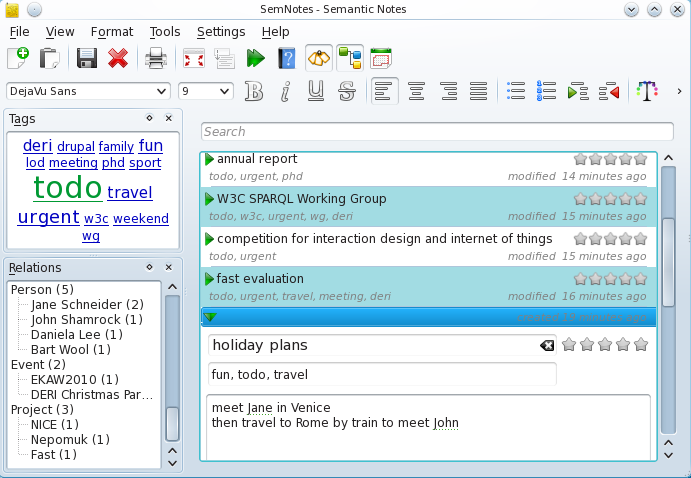
\includegraphics[width=\linewidth]{chapters/core/img/semnotes-screenshot}
\caption{Current version of the SemNotes user interface.}
\label{fig:screenshot}
\end{figure} 

\begin{figure}[tb]
 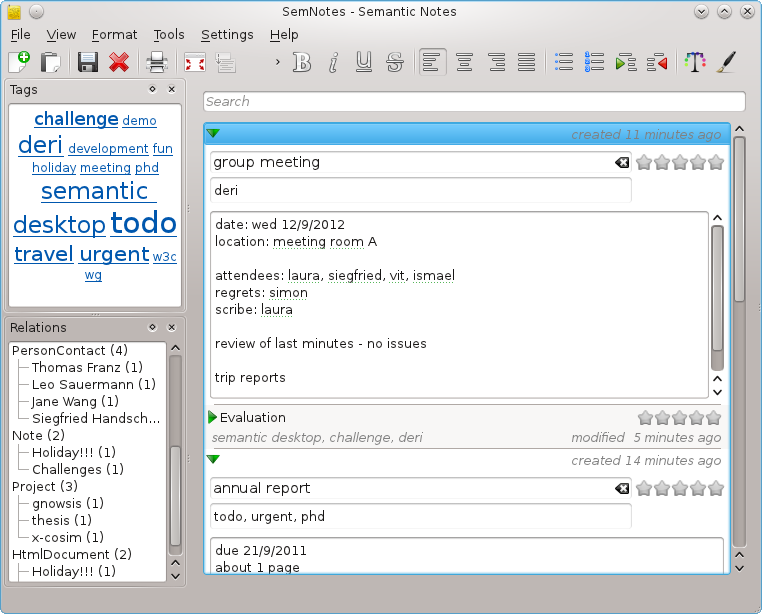
\includegraphics[width=\linewidth]{chapters/core/img/semnotes-screenshot_2notes}
\caption{SemNotes main window, with two notes open in-list.}
\label{fig:screenshot2notes}
\end{figure} 

An aggregated view of the list of notes is based on a restricted set of properties that the notes have in common. Depending on the set of properties used (one or more), the most suitable visual representation of the aggregated view varies. Currently SemNotes offers a tag cloud, a timeline and a related-resource view; each view aggregates information about the notes based on a single property (i.e. the tags associated, the creation date and the related resources, respectively). Aggregated views are displayed adjacent to the list of notes, and can be hidden by the user to allow more space for editing. 

These views also act as a custom faceted browser, as they provide filters on the list of notes. Filtering the list is as easy as clicking on a tag, time interval or related resource. A full text search box also acts as a filter on the list of notes, highlighting the search keywords in the content of open notes, if found. Multiple filters can be set at once, of mixed types. Figure~\ref{fig:screenshot} shows SemNotes with the tag cloud and related-resources views visible, and a tag filter set. A note is open in-list for editing. 

The editor component provides rich text editing of the note content, as well as easy editing of the note metadata. Tagging provides auto-completion based on all the tags on the Semantic Desktop, and creating a new tag is done just by typing its label. If the user does not set a title, SemNotes automatically sets it to the first line of the note. For the rating we used the default visualisation provided by the Nepomuk-KDE libraries, for a uniform interface across the desktop. The creation and last modification dates are the only metadata which cannot be changed through the user interface of SemNotes, as these properties are set automatically. They can be tweaked by expert users, by accessing the RDF repository directly. 

The suggestions for annotations are presented in a simple non-intrusive way, in the ``spell-checker'' style (i.e. the words for which suggestions were found are underlined with a green dotted line instead of a red squiggly line), and are available as context menu items, by right-clicking. Figure~\ref{fig:annotation} depicts how annotation suggestions are presented, and how a linked resource is displayed in the note. To remove an annotation is just as easy as creating it --- through a context menu item.

This presentation of the suggested resources is the result of several iterations of design, each improving on the previous one. 

\begin{figure}[tb]
 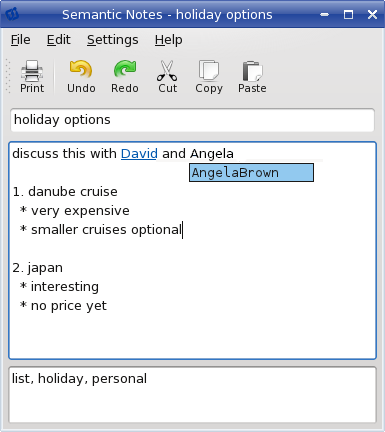
\includegraphics[width=0.6\linewidth]{chapters/core/img/linkednote_v1}
\caption{First version of the SemNotes note editor with pop-up style annotation suggestion.}
\label{fig:popup}
\end{figure} 

The first iteration relied on localised pop-ups with labels of the suggested resources, in the style of text auto-completion (see Figure \ref{fig:popup}). The style worked well when typing the text, and it also enhanced the speed of writing through the auto-completion it provided. The type of annotation of the text during its creation is called latent annotation \cite{Davis2010}, and it is an improvement over the two-step process of first creating the content and then annotating it. Depending on the text of the note, the pop-ups could appear often and distract the user, but they could be dismissed by continuing to type. However, when portions of text were pasted in the editor, several pop-ups were generated at the same time, which was confusing and did not allow the users to make all the connections they would. Changing slightly the pop-ups to only be displayed one-by-one when text was pasted proved not to be a good solution either, as in the case of large paragraphs it would take a long time and many mouse 
clicks for the paste operation to finish, thus interfering with the flow of work. 

Not just the interlinking support was changed from the first version of the application, but the entire user interface. The major redesign was supported by a usability study done as part of the Season of Usability\footnote{\url{http://openusability.org}} 2009, by Daivee Patel, a Human-Computer Interaction student at Drexel University, Philadelphia, USA, with the mentoring help of usability expert Paul Hibbitts of Hibbitts Design, Canada\footnote{\url{http://paulhibbitts.com}}. 
The goals of the project were to recommend changes to improve and/or redesign the SemNotes user interface based on analysis and user research methods, and to perform a usability evaluation of the new changes with a range of users to validate the design recommendations. 

The initial step of the project aimed at forming an understanding of what activities and tasks a user would perform with a note-taking application. This led to the use of a specific technique of task analysis called the activity grid based on the Activity Centred Design methodology. Using this method, we obtained a list of possible activities associated with using a note-taking tool, and each activity was subdivided into the tasks required to perform that activity and each task could then be further subdivided into possible actions. As the tasks became clearer, we identified the tasks that were relevant to SemNotes. These tasks helped focus the effort on the main usability issues and design specifically to address existing issues. 
A comparative analysis of five popular note-taking applications was conducted to help build a knowledge base for reference during the usability inspection of SemNotes. Each of the applications had their own unique features yet certain key functionality appeared standard across these kinds of applications. The examination proved helpful in determining the elements for redesign of the interface. 

The usability inspection of SemNotes was performed to identify usability issues with the existing interface that could be captured without the need to user test before the redesign.
Since the redesign was going to be based on key tasks or activities, we used a heuristic evaluation to identify top level issues.
The criteria for evaluation was the ISO standard ISO 9241\cite{ISO9241}, the principles associated with this standard are based on research and have the benefit of international consensus.
The results of the evaluation were used to help identify areas in the user interface most in need of design improvements, and to create a set of low fidelity mockups. 

A series of usability tests were conducted using the paper prototyping method to validate the initial recommendations for the interface redesign. During each testing session, participants were asked to think aloud and point to elements on the illustrated paper-based screen that they would click or look at based on the tasks provided. No assistance was provided to the users during the testing sessions. The usability test participants were selected via a screening survey on the criteria of experience with computer-based note-taking applications and note-taking habits. 
Based on the feedback from the first set of four users, the mockups were revised for the second round of usability testing while the tasks remained the same. The designs were further enhanced based on the 
feedback received in the second round. 

\begin{table}[htp]
\centering
\ra{1.3}
\begin{tabular}{p{0.45\linewidth} p{0.45\linewidth}}
\toprule
\textbf{Recommendation} & \textbf{Rationale} \\

\midrule
Multi Document Interface (presented as a single window with multiple panes) & By providing all key functionality within a single window, users did not have to manage multiple application windows.\\

Retain optional linking of text within linked editor via use of existing functionality (to click outside the auto complete pop-up) but to be supported by use of icons to indicate the type of resource being linked too & Users showed concern over unwanted text being linked. \\

Search should support searching by tags  & Users realised that since the notes were already tagged during creation, they would like to search by tags for better results. \\

Sorting of notes and tags in the left pane & Multiple options for sorting would help users in locating specific notes and/or tags. \\

First user experience should be provided & Learning curve associated with new applications -- having some introductory information and instructions in the opening screen will be useful. \\

\bottomrule
\end{tabular} 
\caption{Final recommendations for the redesign of SemNotes user interface, based on the usability study.}
\label{tab:sourecommendations}
\end{table}

Based on the accumulated results and feedback, we created a high fidelity mockup of the design, which included all the recommendations (see Table~\ref{tab:sourecommendations}) made as a result of the project, and which were incorporated in the second version of SemNotes.
The next iteration of the display for the annotation suggestions featured a side panel for each of the note edit boxes (see Figure \ref{fig:sidepanel}). The side panel proved to create less interference with the user's workflow, although the suggestions became less obvious. The panel presented the suggestions as a list of resources, that when clicked would highlight the parts of the content to which they were relevant. This helped the users understand from where the suggestion stemmed and if it was indeed correct. To create a link between the note and a suggested resource, the user had to right click on the corresponding item in the list and select ``Link''. Resources could also be removed from the suggestion list, and never be shown again for the current note, to help clear the list from overpopulating. This interface shifted the initial latent annotation style of SemNotes, back to a classic two-step process. Although the suggestions were still computed on the fly, as the user typed or pasted new text, 
because they were out of focus, users were inclined to leave the annotation step for later. Another issue of the side-panel variant was that it limited the screen real-estate for the most important function of SemNotes, that of note-taking. 

\begin{figure}[tb]
 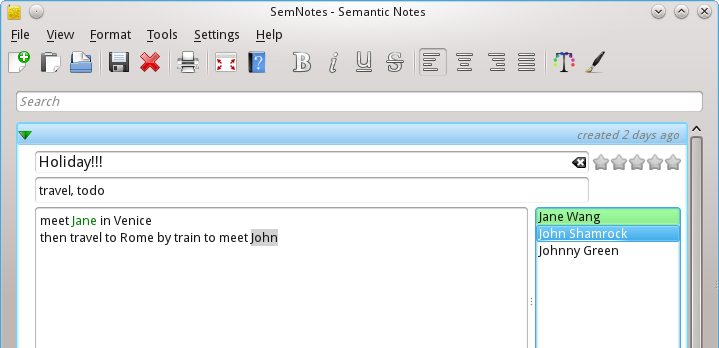
\includegraphics[width=\linewidth]{chapters/core/img/linkednote_v2}
\caption{Second version of the SemNotes note editor with a side panel to display the annotation suggestions.}
\label{fig:sidepanel}
\end{figure} 

To keep more of the screen space for the note editor, in the next iteration, we have abandoned the side panel in favour of the ``spell-checker'' type of notification. It is a mix of the first and second iterations, by giving the users the immediate feedback of the pop-ups, through the green dotted line that underlines words, while being unobtrusive in the note-taking activity. The suggestions are computed on-the-fly like before, but they are only shown if the user right-clicks on the underlined word or words, in keeping with the spell-checker metaphor.

The three iterations of user interface design have improved significantly the usability of SemNotes, as well as the ease of interlinking. However, further usability testing is needed to determine whether and how different types of relations can be created between the notes and the related desktop resources. 


\section{Evaluation}
\label{sec:semnotesevaluation}

We conducted a task-based summative user evaluation, comparing SemNotes to the popular note-taking application Evernote\footnote{\url{http://evernote.com/}}. The goal of the experiment was to determine whether the effort required for the creation of links between notes and resources is repaid by easier search. Towards this goal, we measured the effort needed to execute the same set of tasks with both tools, and compared the results. We used time spent, number of mouse clicks and number of key presses, as measures for effort. After the experiment, we asked the participants about their experience in a questionnaire.

The two applications compared have the same main functionality, note-taking. We chose Evernote as baseline, as it is a very popular note-taking tool that is freely available. Its set of functionalities are richer than those of SemNotes, but the basic features are present and similar in both applications. The feature that distinguishes SemNotes is the same that we want to measure---the creation of links between the notes and desktop resources, based on suggestions given by the application. SemNotes runs on KDE on Linux, and uses the framework provided by Nepomuk-KDE Semantic Desktop. Evernote runs on several operating systems for desktop and mobiles, but Linux is not one of them, therefore we used its Windows version. 

Evaluation is one of the challenges for application design on the Semantic Desktop. Adding to the challenges of evaluating PIM applications with regards to finding appropriate data and tasks for significant measurements, discussed in \cite{Kelly2006}, semantic PIM applications have the difficulty of lacking equivalent semantic tools for a one-on-one comparison. That is why for this evaluation, we followed a methodology similar to the ones described in \cite{Elsweiler2007} and \cite{Franz2009}, of comparing our semantically enabled SemNotes, to a conventional application.

One aspect that we did not evaluate as part of this study is the effect of having the notes connected to the relevant desktop resources from the other applications using the respective resources --- for example, would the extra information from the notes provide an advantage when using a task manager application, and seeing all the linked notes when looking at a task. Such a study would require a longer duration, and also a richer ecosystem of semantic applications, which make use each other's data.

\subsection{Participants} 

Twenty participants took part in the evaluation, all members of our research institute. They are researchers in the field of Semantic Web, thus possibly favouring the semantic application. This bias (if it exists) would however influence only their responses in the questionnaire and not the measured values. Fourteen participants regularly use note-taking and five of them use Evernote as their preferred note-taking tool. None of the participants used Linux as their operating system. Their familiarity with one environment and one application could have influenced the measured results, in favour of Evernote.

\begin{figure}[htb]
 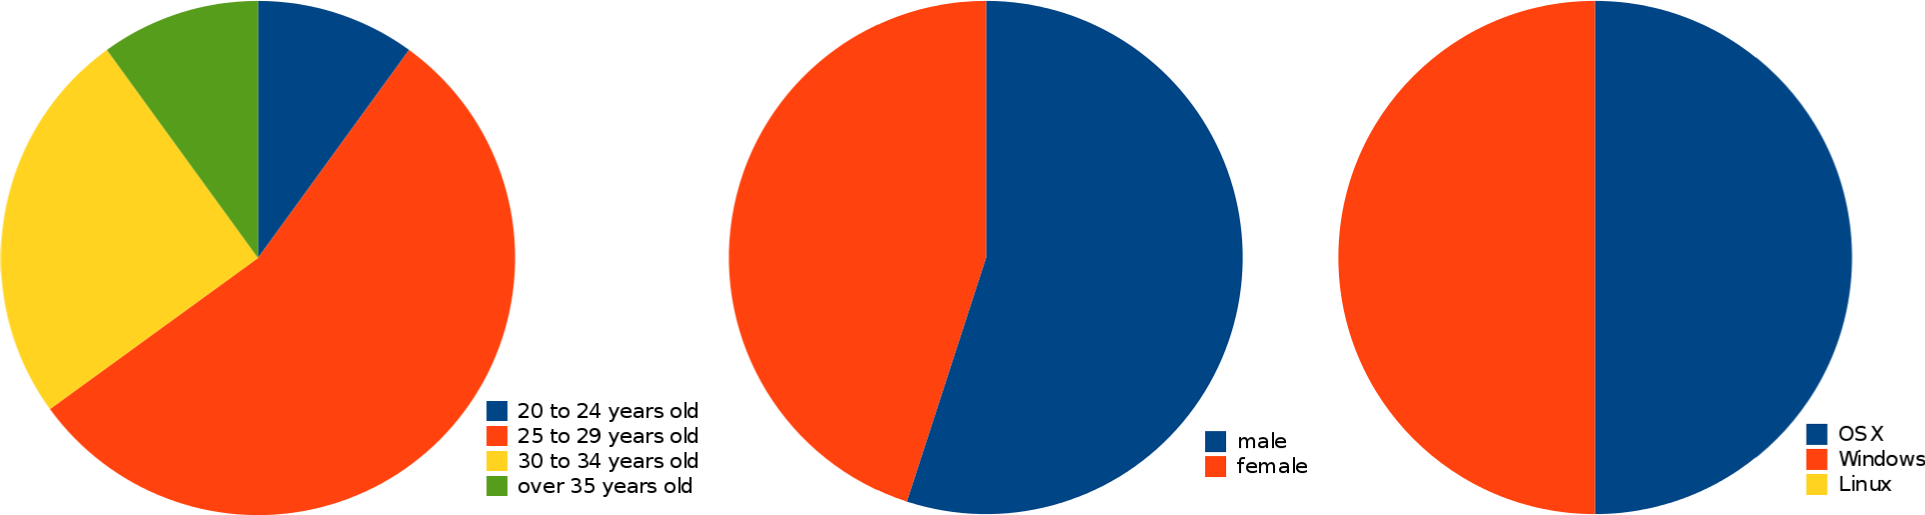
\includegraphics[width=0.95\linewidth]{chapters/core/img/distribs}
\caption{Age, gender and OS distributions of participants.}
\label{fig:distribs}
\end{figure}

Some additional demographic details of the participants: gender distribution was close to even (eleven men and nine women); most of them were in the age groups between 25 and 29 (eleven, equivalent to 55\%), and between 30 and 34 (five, or 25\%). There were seven Master's students, seven Ph.D. students, five senior researchers and one intern. For demographic distributions see Figure \ref{fig:distribs} and Figure \ref{fig:genderdistribs}.

\begin{figure}[htb]
 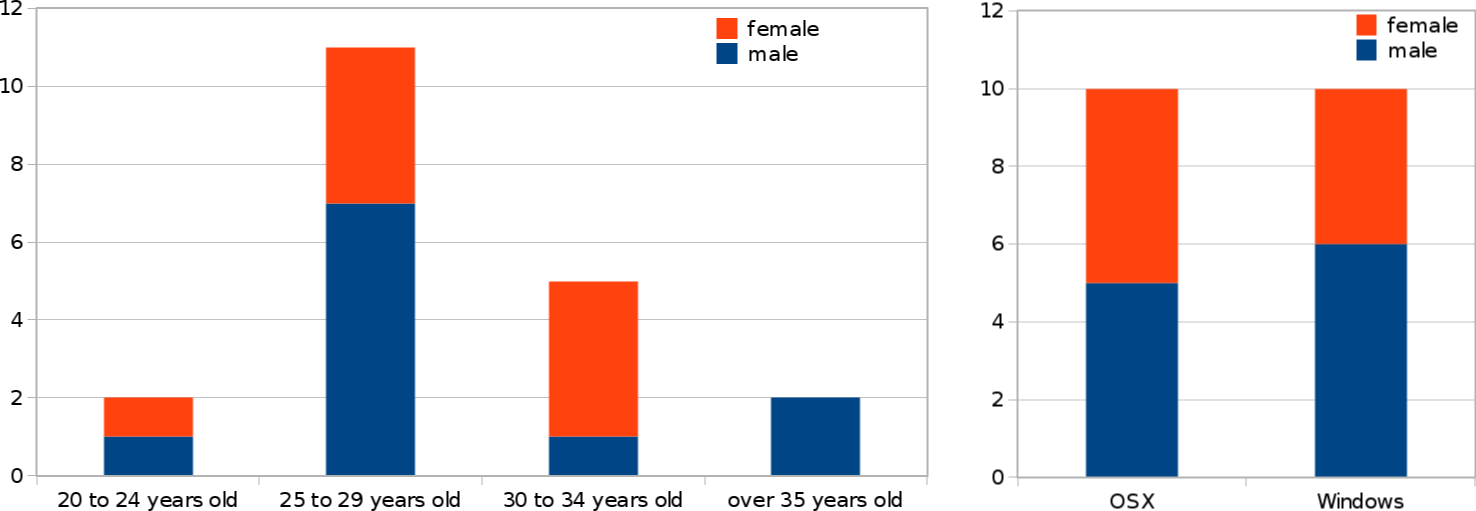
\includegraphics[width=0.9\linewidth]{chapters/core/img/genderdistribs}
\caption{Age and OS distributions of participants per gender.}
\label{fig:genderdistribs}
\end{figure}

\subsection{Data} 

We used two virtual machines for the experiment, preloaded with identical data. To reduce the artificialness of the study, we chose general data familiar to the participants, to which they have access in their everyday work. The dataset contained contact information for 130 members of our institute; 655 recent emails from our mailing lists; 20 scientific papers authored by our colleagues; and photographs from institute events. The note data was also identical: 50 notes on a variety of topics, personal or work-related, tagged with 23 tags. In SemNotes, we also provided links between the notes and the resources mentioned in them: people, projects, events or other notes, within reasonable limits we expect users to interlink their notes (i.e. minimum 0 links, maximum 10 links, average 1.8, median 1). The majority of connections were made to people mentioned in the notes.

\subsection{Tasks} 

We prepared a set of eight tasks. Each participant was requested to run all the tasks in each of the two environments. To prevent order effects from influencing the results, half of the participants started with SemNotes and the other half with Evernote.

\begin{description}
 \item[T1.] Find what information is available about yourself (contact information, documents, emails, photographs)
 \item[T2.] Find the paper titled ``Bridging the Gap between Linked Data and the Semantic Web''. Who are the authors?
 \item[T3.] Find notes tagged with ``todo''.
 \item[T4.] Find to-dos that are related to our institute.
 \item[T5.] Find a to-do related to a presentation by a colleague John.
 \item[T6.] Take a note about planning a social event for your research group. Write the names of two people that have already confirmed. Annotate the note as you see fit.
 \item[T7.] Find a note containing the minutes from the last meeting about a given project. Change the date of the next meeting planned.
 \item[T8.] Take a new note for the action item assigned to you at the last meeting of the project. The action item is in the meeting minutes previously edited, and it requires drafting a document using a paper authored by a colleague. Annotate the note.
\end{description}

The first two tasks were intended to help the participants get accustomed with the data available and the environment; we did not include the time spent on these tasks in the results. 

The last six tasks were focused on note-taking, and their complexity increased gradually. T3, T4, and T5 are search and filter tasks (S), from the very simple to the complex. T6 and T8 are editing tasks (E), including any annotations that the participants made on the notes. T7 is both a search and edit task (SE). It prepares the participants for the most complex search and edit task, T8, which required interaction with the rest of the system (i.e. finding the required paper).

\subsection{Measurements} 

The participants were recorded while doing the tasks of the experiment, and the videos were used to extract the measurements used in the analysis. 
For each task we measured the effort in seconds spent, and number of mouse clicks. 
We also counted the number of key strokes for the tasks involving creation of notes, and we used this measure to normalise the values for time. 
Although we had two separate measures for each task, we were interested in the difference between these values, computed according to:
$$
value_{difference} = value_{SemNotes} - value_{Evernote}
$$
Thus, a positive value means that the value recorded for SemNotes is bigger than the corresponding value for Evernote, and a negative value means that the value for SemNotes is smaller. 

For the time measurements, the time difference represents the extra \emph{effort} required for annotating the notes with links in the editing tasks. For the search tasks the difference shows which of the applications enables the users to find the notes easier, thus the \emph{benefit}. We must specify here that actual searches done by the software were considered instantaneous, as the datasets are small and we did not intend to measure the performance of the search algorithms used.

For the number of mouse clicks, the difference represents the extra \emph{effort} required, for both types of tasks.

\begin{figure}[tb]
\begin{center}$
 \begin{array}{ccc}
  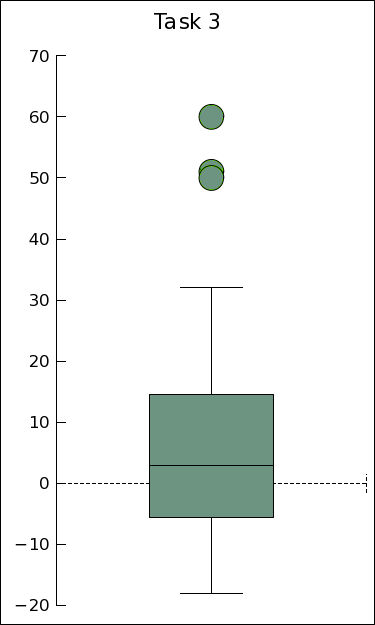
\includegraphics[width=0.29\linewidth]{chapters/core/img/task3difboxplot} &
  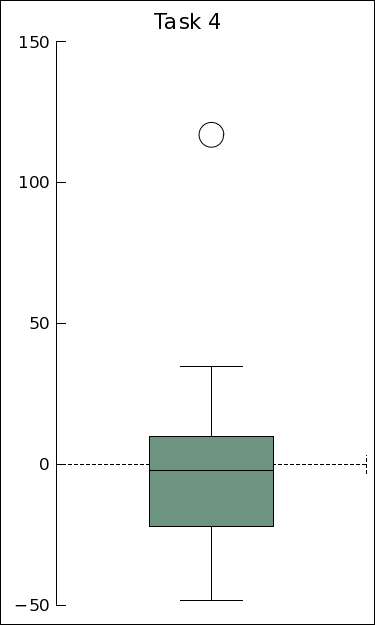
\includegraphics[width=0.29\linewidth]{chapters/core/img/task4difboxplot} &
  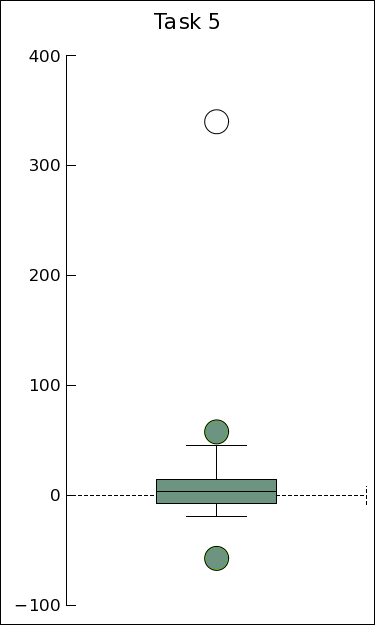
\includegraphics[width=0.29\linewidth]{chapters/core/img/task5difboxplot} \\ 
  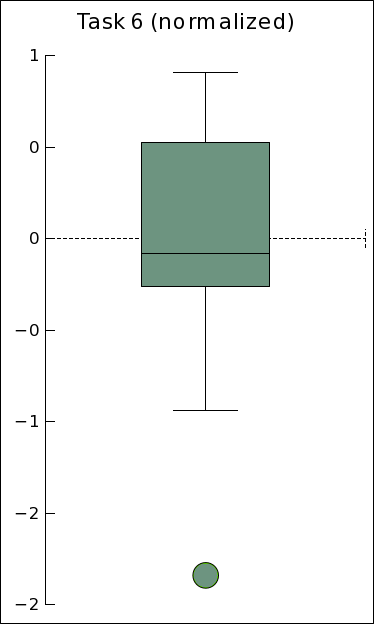
\includegraphics[width=0.29\linewidth]{chapters/core/img/task6difboxplot} &
  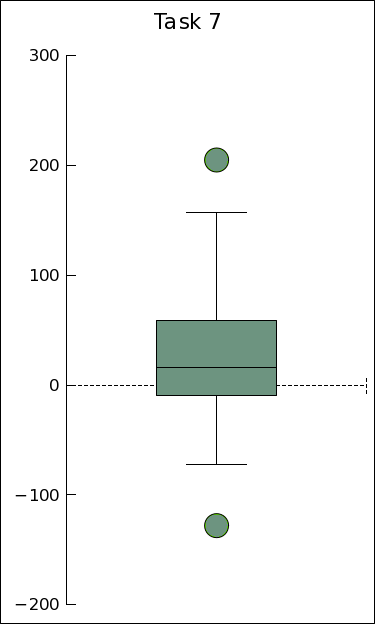
\includegraphics[width=0.29\linewidth]{chapters/core/img/task7difboxplot} &
  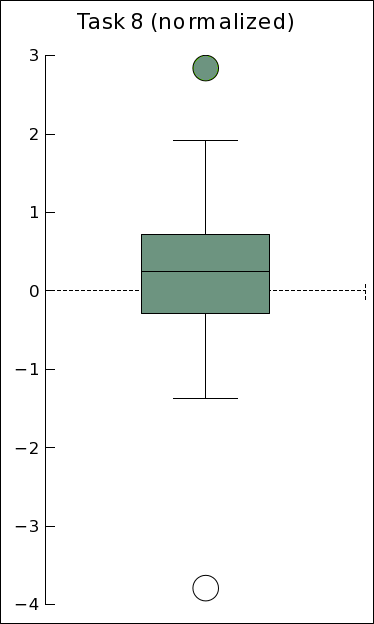
\includegraphics[width=0.29\linewidth]{chapters/core/img/task8difboxplot} 
 \end{array}$
\end{center}
\caption{Inter-quartile ranges for the time difference.}
\label{fig:boxplots}
\end{figure}

After a first analysis of the results, we noticed that some values for time were unrealistically high or low. They coincided with the measurements when the participants stopped to ask a question or comment on a feature. We decided to eliminate these outlier values by using only the measurements that fall in the inter-quartile range, for all tasks --- see Figure \ref{fig:boxplots}.

\subsection{Quantitative Results}

We tested if the effort measured in time and mouse clicks was different when using SemNotes than when using Evernote. Table \ref{tab:semnotesresults} shows the results, with the statistically significant values in bold (\begin{math}p < 0.05 \end{math}).

\begin{table}[htp]
\centering
\ra{1.3}
\begin{tabular}{@{}clcr@{.}lr@{.}lr@{.}lcr@{.}lr@{.}lr@{.}l}
\toprule
\multirow{2}{*}{\textbf{T}} &&& \multicolumn{6}{c}{\textbf{Time (s)}} && \multicolumn{6}{c}{\textbf{Clicks}} \\

&&& \multicolumn{2}{c}{\textbf{Avg}} & \multicolumn{2}{c}{\textbf{Med}} & \multicolumn{2}{c}{\textbf{\textit{t}}} && \multicolumn{2}{c}{\textbf{Avg}} & \multicolumn{2}{c}{\textbf{Med}} & \multicolumn{2}{c}{\textbf{\textit{t}}} \\
\midrule
\textbf{T3} & (S) && 0 & 5 & 0 & 0 & 0 & 152 && 0 & 167 & 0 & 0 & 0 & 692 \\

\textbf{T4} & (S) && -8 & 0 & -8 & 0 & \textbf{-2} & \textbf{94} && -0 & 333 & -1 & 0 & -0 & 48 \\

\textbf{T5} & (S) && -0 & 125 & 1 & 0 & -0 & 046 && 0 & 857 & 1 & 0 & 1 & 426 \\

\textbf{T6} & (E) && 0 & 063 & 0 & 016 & 0 & 486 && 6 & 067 & 8 & 0 & 2 & 026 \\

\textbf{T7} & (SE) && 14 & 357 & 13 & 0 & 1 & 713 && 4 & 812 & 2 & 0 & 1 & 527 \\

\textbf{T8} & (SE) && 0 & 249 & 0 & 243 & 1 & 004 && 20 & 8 & 12 & 0 & \textbf{3} & \textbf{08} \\

\bottomrule
\end{tabular} 
\caption{Statistics for time and click differences.}
\label{tab:semnotesresults}
\end{table}

Results show that for the simple search task T3 the difference is positive, which suggests that it takes longer to finish the task with SemNotes. However, the difference is not significant. For the complex search tasks that follow, T4 and T5 the difference has negative values, showing that the users spent less time on complex searches when using SemNotes, thus supporting the claim that the use of interlinked data makes notes easier to find. Only the results for T4 are statistically significant. None of the measures of number of mouse clicks for the search tasks are statistically significant, the differences being in average less than 1 click, with a median value of 0, -1 and +1 respectively for the tasks T3, T4 and T5.

For the editing task T6, the values are positive, thus it took longer to finish it with SemNotes. This was expected, as in SemNotes there is the additional step of annotating the notes with links to desktop resources. However, the differences are very close to 0 (0.063s average and 0.016s median) and not statistically significant. This editing task did require in average 6 more mouse clicks in SemNotes, with a median value of 8, but the difference is also not statistically significant.

For the more complex search and edit tasks T7 and T8, the time differences, while positive, thus in favour of Evernote, are not significant. For both tasks the values were positive, which mean more clicks when using SemNotes. However, task T8, that required creating and annotating a complex note based on information from other sources, had statistical significant difference in number of clicks, in favour of Evernote (more clicks needed in SemNotes). 

The positive difference in the number of clicks required for all editing tasks (T6, T7 and T8) is not surprising, as the participants recognised the value of creating links and proceeded to link the new note to the relevant resources. This was however a motivation for providing better keyboard support for the annotation of notes in the future version of the tool.

In summary, the results show that there are significant improvements (for one of two tasks) in the time spent on complex searches, when the data is interlinked, at no significant extra cost for the creation of the links. Linking does however significantly increase the effort measured by number of mouse clicks (for one of two tasks).

\subsection{Questionnaire}

We asked the participants to fill in an anonymous questionnaire related to the experiment. The questionnaire is listed in Appendix~\ref{ap:questionnaire}. According to the answers, on a scale from 1 to 5, the tasks were simple (mean 2.25) and similar to the ones in their daily work (mean 3.4), and the data provided was familiar (mean 3.2). 

The answers also show that 60\% of the participants (12) felt that SemNotes helped them finish the tasks \emph{faster}, while only 20\% (4) said Evernote, and 20\% did not feel any difference between the tools. When asked which of the two applications helped them perform the tasks \emph{better}, 80\% of the participants chose SemNotes, while the remaining 20\% did not feel that there was any difference (see Figure \ref{fig:betterfaster} for a graphical representation).

\begin{figure}[htb]
 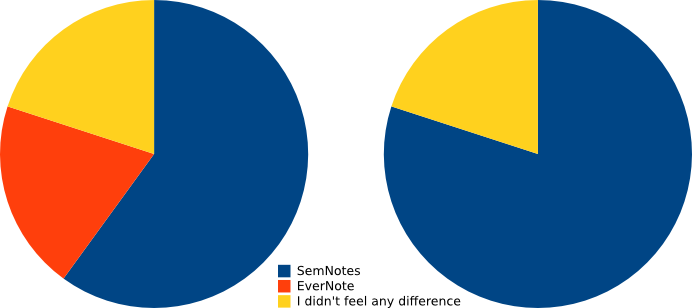
\includegraphics[width=0.7\linewidth]{chapters/core/img/fasterbetter}
\caption{Which tool helped perform the tasks faster (left) and better (right).}
\label{fig:betterfaster}
\end{figure}

The participants had a good overall impression of SemNotes (with a mean of 4.15 on a scale from 1 to 5). This rating was supported by comments like ``\emph{That was cool.}'', and requests for SemNotes for other operating systems: ``\emph{Maybe you could make an OS X version?}'' and ``\emph{When is a port for Windows 7 coming?}''.

The semantic annotation was one of the most liked features of SemNotes, and one of the features most missed in Evernote, according to the questionnaire. Another advantage of SemNotes was considered the multiple filtering by mixed criteria, with several participants considering it the best feature. The rating of notes was listed as the least liked feature of SemNotes by three participants. The tag cloud was the most controversial feature, as many participants liked it and found it very useful, while others would have preferred a simple list of tags: ``\emph{Usually I don't like tag clouds, but the one in SemNotes was really useful.}'' and ``\emph{While the tag cloud helps in determining the most used tag, a simple list with the tags seems to be easier to search.}'' 


\section{Related Work}
\label{sec:notetakingapps}

Semantic note-taking means enhancing the note-taking process using Semantic Web technologies. It can refer to the techniques and methods used in the implementation, like ontologies and RDF, but most importantly it is about creating a semantic network around the notes and the information contained in them. There are several applications that enable more or less semantic note-taking: some are browser based (online or offline), while others are standalone desktop applications as is SemNotes. 

The List.it browser-based note-taking tool \cite{Kleek2009} and Jourknow, its predecessor \cite{Kleek2007}, save context alongside the information scraps, to improve re-finding and reminding. List.it also features information extraction from the unstructured text of the notes, recognising entities and relations between them, with the \emph{pidgin} language processor. However, unlike SemNotes, the contex of the notes they create does not include links to any existing desktop resources. SnapShoot \cite{Iga2006} is another browser-based note-taking tool that explores new visualisation techniques to improve reading of the documents produced. It features categorisation, and limited interlinking with documents within the system.

MindRaider \cite{MindRaider}, described above in Section \ref{sec:sdsystems}, is an open source ``Semantic Web outliner'' and extended note-taking system for information organisation. While it only interlinks concepts within its maps, it can connect to the Gnowsis Semantic Desktop through a plugin, thus potentially it can use any Semantic Desktop resources through a similar mechanism.

A distinct category of semantic note-taking applications are personal semantic wikis, like Kaukolu \cite{Elst2008}, IkeWiki \cite{Schaffert2006} and GDKTiddlyWiki. Each wiki page represents a resource and its semantic relations to other resources are encoded within the page, using an extension to the wiki syntax. Only predefined relations and types are available, and the wikis offer limited access to other desktop information sources. Unlike SemNotes, connections are only possible between resources within the wiki system.

OneNote from Microsoft's office suite provides quasi-se\-man\-tic functionality by interlinking the notes with address book information, calendar, and tasks. It does not use any semantic technologies though, and the data is locked in by proprietary formats and storage.

Zemanta\footnote{\url{http://www.zemanta.com}} is a blog assistant that suggests possible enhancements to blog posts, like linking external content and images. Unlike SemNotes, which uses the local repository to search for matches, Zemanta looks on the Web. It does not assign any semantics to the links. 

There are also specialised systems like the SemanticPen \cite{Varadarajan2005} which provides support for semantic note-taking with pen devices.
Other note-taking applications that provide semantic features include: Jenga Note\footnote{\url{http://www.jenganote.org}} --- allows associating a note with a concept, Catch Notes\footnote{\url{http://www.catch.com}}, and SpringPad\footnote{\url{http://www.springpadit.com}}.


\section{Conclusion}

In this chapter, we presented a solution to the challenges of designing applications for the Semantic Desktop. We described one such application, SemNotes, a semantic note-taking tool for the Nepomuk-KDE Semantic Desktop. It provides a real-world, functional use case for fully exploiting the capabilities of the Semantic Desktop: interlinking, organisation and management of personal information, efficient search and browsing. It supports the entire life-cycle of the semantic data represented by notes, with emphasis on the creation of links between the new data and the existing network of linked information on the desktop. 

Through SemNotes we present a possible solution to each of the challenges presented in the begining of the chapter. To the first question of creating semantic data, we describe how we create new semantic notes, using the existing vocabularies and creating links to the existing Semantic Desktop data available. To the second question of designing the human computer interaction, we describe the efforts towards an easy to use yet rich user interface design for SemNotes. With the help of usability experts and user testing the interface went so far through three iterations, each described in this chapter.

For the third challenge, that of evaluating a semantic tool, we described a task-based user evaluation comparing SemNotes to the popular note-taking application Evernote. The results show that the extra effort (measured in time spent) required for the annotation of notes with links to related resources is not significant. However, the benefit (measured in time saved) is significant for one of two complex search tasks. 

SemNotes embodies a simple and user-friendly way of generating new semantic data on the desktop, and integrating it with the already existing data. However, the personal information that the users work with is not restricted to the desktop. Further, semantic data exists in large quantities outside of the desktop, on the Web and in organisational repositories. Thus, in the next chapter we continue by describing how the linked information from the desktop can be meaningfully and safely connected to the outside world.


\chapter{Bridging the Gap between the Semantic Desktop and the Web of Data}
\label{ch:sdwod}

\begin{flushright}
 \textit{Based on ``Linking Semantic Desktop Data to the Web of Data'' \cite{Dragan2011b}\\published at the 10th International Semantic Web Conference (ISWC~2011)}
\end{flushright}

The previous chapters showed how the Semantic Desktop enables better personal information management on our computers, using semantic technologies to explicitly connect information which is naturally connected in the real-world, and thus matching the representation to a user's mental model. However, our personal data is often a reflection of our subjective view, or limited knowledge. Thus, although it may seem huge when faced with the task of organising it, the information on the desktop is small compared to the amount of information available online. The Web of Data contains a linked network of information similar to the one on the desktop, only at a much larger scale. Connecting the desktop to the Web of Data would enrich and complement desktop information.

This chapter presents a solution to the second research question \textbf{Q 2.} from Section \ref{sub:question}, \emph{how to expand the scope of the Semantic Desktop into the realm of the Web of Data, to enhance the user experience and benefit?}, more specifically, to the first sub-question \textbf{Q 2.1.} described there --- \emph{how to find instances representing the same real-world thing described by a Semantic Desktop resource?}

Our solution uses a semantic search engine for the Web of Data, such as Sindice\footnote{\url{http://sindice.com/}}, to find and retrieve a relevant subset of entities from the Web. We present a matching framework, using a combination of configurable heuristics and rules to compare data graphs, that achieves a high degree of precision for the linking decision.
We evaluate our methodology with real-world data --- we create a gold standard from relevance judgements by experts; and measure the performance of our system against it. We thus show that it is possible to automatically link desktop data with Web data in an effective way.

\section{Introduction}
\label{sec:sdwodintro}

The Semantic Desktop aims to enable better organisation of the personal information on our computers, by applying semantic technologies on the desktop. Just as Linked Data connects distributed data on the Web, creating a network of interlinked information, the Semantic Desktop connects personal data across application boundaries on the desktop, creating a network of personal information.
However, information on our desktop is often incomplete, as it is based on our subjective view, or limited knowledge about an entity.

On the other hand, the Web of Data contains information about virtually everything, generated by multiple sources, and theoretically unlimited. Connecting the desktop to the Web of Data would thus enrich and complement desktop information. Bringing in information automatically from the Web of Data would release the user from the burden of searching for information.

Connecting the two networks of information opens up the possibility of personal services on the desktop, which use external data but in the personal context of the user, highly connected to his personal data and focused on his interests. One such example is a service that finds implicit links between the publications that the user has on the desktop, and provides recommendations to other publications on the same topics, by the same authors, or related in another way. 
Another desktop service could use information from the Web of Data to notify the user of new concert dates in his area, based on the latest or most popular artists played on the desktop. 
Web data can also be used as a point of reference when working collaboratively, e.g., documents linked by the user to people, projects, or other resources from his semantic desktop can be shared together with the annotations, which can be accessed and reused outside of the Semantic Desktop where they were generated.

From the perspective of interlinking information, and using the frameworks provided by the Semantic Desktop and the Web of Data, we have separate islands of knowledge, both containing similar data, related to the same topics of interest to the user, but disconnected from each other. 

The disconnection appears in two forms:
\begin{itemize}
 \item The data on the desktop, although similar to that on the Web of Data, is described using specific \emph{desktop ontologies}, which are different from the ones found on the Web of Data. This schema mismatch makes interlinking data from the two datasets difficult.
 \item Identifiers (URIs) on the desktop are local to the desktop data space, they are not globally unique and cannot be dereferenced as normal Linked Data URIs are. Hence, it is hard to access and connect to local data from the Web.
\end{itemize}

To tackle this disconnection, it is necessary to create links between desktop identifiers and Web identifiers that refer to the same real-world thing.
This means we need to compare the data graph describing an entity on the desktop with the data graph of an entity on the Web. Leaving aside the use of different terminology within the data, the Web of Data is large, with billions of entities across hundreds of thousands of datasets. From this vast amount of information we must find and retrieve a relevant subset of entities, that are potential candidates with the desktop entity. Then we must decide if the candidates are similar enough with the desktop entity to create a link between the two. Because we wish to make the interlinking automatic, we must be able to decide with a high degree of precision which candidates among this subset are in fact referring to the same entity.

Our solution tackles the problems raised above by using a semantic search engine for the Web of Data, such as Sindice, to find and retrieve
a relevant subset of entities from the Web. We then present a matching framework, using a combination of configurable heuristics and rules to
compare data graphs, that achieves a high degree of precision in the linking decision. 

To evaluate our methodology with real-world data, we create a gold standard from relevance judgements by experts, and we measure the performance of our system against it.

Our solution proves that interlinking the two environments is feasible, and even more, it yields good results. Connecting desktop data with the Web enables the system to bring Web data to the users, instead of the users having to go find it by themselves.


\section{Related Work}
\label{sub:sdwodrelatedwork}

The problem of entity linking is well known across various research communities with a variety of different names, such as record linkage \cite{Felligi1969}, entity resolution \cite{Benjelloun2006}, reference reconciliation \cite{Dong2005b} or object consolidation \cite{Hogan2007}. A wide variety of algorithms has been developed for resolving the co-reference problem, but record linkage between distributed databases is still considered a  difficult problem.

Recent initiatives within the Semantic Web community address the problem of linking entities across data sources. For instance, \cite{Jaffri2007} describe the phenomenon of proliferation of URIs and propose a Consistent Reference Service to manage URI equivalences. The OKKAM project \cite{Bouquet2007} proposes an infrastructure for assigning global identifiers at web scale. These approaches are more focussed towards the management of entity identity on the Web, but do not provide an easy means to create new links between data sources. 

Similar to our approach, \cite{Raimond2008} describe an algorithm and its implementation GNAT, for linking a personal music collection to corresponding MusicBrainz resources. The approach recursively measures the similarity of the resource graphs from the two datasets, with the limitation that the same vocabularies must be used in both. By contrast, using property paths in our mappings, we eliminate the need for recursion while still propagating the measures from connected resources.
Silk is a framework for linking multiple entities between two datasets \cite{Bizer2009}. It relies on user-defined rules and various string matching algorithms to measure the similarity between two entities. In this case it is necessary to know a priori which specific dataset to link to and to perform manual configuration of the matching algorithms, something that requires a high degree of expertise.
\cite{Hogan2007} and \cite{Sais2007} propose logic-based methodologies for merging identifiers of equivalent entities across multiples knowledge sources. While being precise, these techniques do not have a very good recall and are computationally demanding.

The most relevant approach related to ours is the Silk framework. We provide a generic matching process that the user can configure based on their own expertise in order to get more precise results. However, our approach differs by the fact that the matching process is not restricted to linking data between two predefined information sources. On the contrary, our approach makes it possible to link desktop data with an arbitrary number of external data sources. This makes the problem harder since we are generally unaware of the data structure or schema of these data sources. 

We therefore need to first find potential entities of interest among a vast number of data sources, then retrieve a partial description of these entities and rely on more complex entity matching algorithms. 

This first step of our algorithm can be seen as a blocking pass to reduce the information space before executing complex matching algorithms \cite{Elmagarmid2007}. The blocking step is implemented on top of a boolean query model for centralised search systems such as Sindice \cite{Tummarello2007} and on top of the SPARQL query language for specific data sources providing a SPARQL endpoint.

\cite{Nikolov2012} propose the use of a genetic algorithm to achieve unsupervised discovery of the similarity parameters needed for data linking between two datasets. Similarly to our algorithm, the approach proposed uses a blocking pass using a SPARQL query, to reduce the computation time. As with Silk, the algorithm considers only two datasets to be matched.


\section{The Process of Finding Web Aliases}
\label{sec:process}

The goal of our algorithm and system is to find Web aliases for desktop resources. A Web alias is a Web entity identifier, i.e., URI, that represents the same real-world thing as the desktop entity to which it was matched. To find Web aliases, we use the information available on the desktop, like the contact information from the address book for people, or metadata of music files for songs, albums and artists. We also use the knowledge about the desktop ontologies and the way data is organised and used on the desktop. The desktop data drives the entire process, and is used throughout the steps:

\begin{enumerate}
 \item Candidate selection --- blocking pass
 \begin{itemize}
  \item Query and identify candidate entities from various Web of Data sources
  \item Retrieve data for each candidate from the appropriate source[s].
 \end{itemize}
 \item Candidate filtering --- scoring based on similarity
 \begin{itemize}
  \item Compute similarity score based on the data of the entities.
  \item Filter the candidates based on the similarity score.
 \end{itemize}
\end{enumerate}

The first step requires identifying a list of candidate entities and obtaining the data available about them. There are two options for this:

\begin{itemize} 
\item through a small set of sources that we know have the data we need, and can query each of them independently for possible candidates, or 
\item through a search engine for the Web of Data, like Sindice \cite{Tummarello2007} which indexes millions of documents containing semantic mark-up.
\end{itemize}
Each option has use cases where it is more suitable than the other, thus we designed our system to support both. Querying specific sources is preferred for instance, if the data is from a very specific domain, like cancer research, or when we are interested only in results from an organisation's internal repository. Using a search engine is best when the information sources to query are not known a priori. It also has the advantage of covering a large number of information sources with only one query, and of selecting the most relevant data sources and candidates with respect to the query via the search engine ranking system. However, in the case of ambiguous entities, the latter option has the disadvantage of returning too many unrelated results, thus making the entity selection more difficult.

Once a list of candidates is available, we compute a similarity score for each of them with respect to the desktop entity. The desktop data is considered authoritative, and the matching process is driven by it. This has the apparent advantage of control, since the desktop data is more strictly under the control of the user. However, there are cases when the desktop data is simply insufficient, or has uncaught errors due to the user's incomplete information, or the Semantic Desktop's extraction process.

The matching algorithm checks first whether the types of the candidate entities correspond to the type of the desktop entity, and discards the ones that do not.
Only then are the data of the entities examined and the properties and corresponding values compared. If required, the algorithm looks at other related entities and their properties. The values of the properties are compared using either exact string matching or string similarity techniques. As mentioned above, the ontologies used on the desktop are different from those used on the Web, thus both type checking and property matching require mappings between the two sets of vocabularies.

After the matching algorithm computes the scores for each of the candidates, the list is filtered for values above a given threshold. References to those Web resources which passed are saved in the desktop repository, as \verb|pimo:hasOtherRepresentation| links from the initial desktop resource.


\section{Implementing the Process}

We implemented the process described above in a desktop daemon that finds Web aliases for desktop entities.
It sequentially searches for aliases for all resources that have no alias listed, and for resources that have changed since the last time aliases were determined for them. In the case when a resource is revisited after being modified, the previously found aliases are discarded and new ones are searched for.

The result of the process is the creation of new links on the Semantic Desktop between local resources and their Web aliases. They can be used to enhance the desktop data about the entities, or as entry points to access further information online.

The implementation has two major components, each handling one step of the matching process: A query component that initiates the search and identifies the candidates, and a matching component that filters the candidates based on similarity measures. We next discuss these components in turn.

\subsection{The Query Component}
\label{sub:querymodule}

The query component was designed to be able to use either generic search engines or specific data sources. Therefore, we chose to make the query module plugin-based, thus allowing various new sources to be connected if needed. The query modules are responsible for finding the initial list of candidates, as well as for retrieving the data for each candidate. The maximum number of candidates to retrieve from a data source can be set as a parameter in the configuration. We allow three types of plugins:
\begin{description}
 \item[SWSE] --- connect to semantic search engines, through their APIs. We provide a plugin of this type for Sindice.
 \item[Sparql] --- connect to sources that provide a SPARQL endpoint. We provide plugins of this type for DBpedia and the Semantic Web Conference Server.
 \item[Custom] --- connect to other sources, possibly ones that do not expose any data as RDF (e.g., relational databases or third-party APIs like last.fm).
 \end{description}

Most major Linked Data providers (e.g. DBpedia) are indexed by Sindice, therefore the Sindice plugin is the only one enabled by default.

In the Sindice module, the initial query, which determines the list of candidates, is constructed using all the value properties of the desktop entity, combined using the boolean conjunction operator ``OR''. Multiple word terms are also tokenised and the tokens are added to the query. This may result into a longer query which contains duplicate words. This is however due to the fact that we rely on the search engine to interpret the query and rank higher the results that match most of the terms. The search engine (in this case Sindice) algorithm ranks higher results which match more of the strings connected by ``OR''. Building the query with just the strings without quotes would result in automatic tokenisation by the search engine, which might lead to higher ranking of unsuitable results, especially if the words searched for are common. Thus we chose to prevent the tokenisation by the search engine by using quotes around the full string searched for, but still mimic the default behaviour of the algorithm by 
doing the tokenisation ourselves, as a fail-safe in case the query yields no results. 

For the music album ``One Night Only'' by the Bee Gees from 1998,  the query constructed is:

\begin{quote}
 \emph{``Bee Gees'' OR ``One Night Only'' OR ``1998'' OR ``Bee'' OR ``Gees'' OR ``One'' OR ``Night'' OR ``Only''}
\end{quote}

\subsection{The Matching Component}
\label{sub:matchingcomp}

The matching module computes a similarity score for each pair $($\emph{desktop~entity}---\emph{web~candidate~entity}$)$. The way the score is computed depends on a set of parameters:

\begin{description}
 \item[String matching (SM)] --- If this parameter is set to \texttt{true}, the matching module will use string similarity measures where appropriate. Currently the system supports Monge-Elkan \cite{Monge1996} and Chapman\footnote{\url{http://sourceforge.net/projects/simmetrics/}} distances. If the value is set to \texttt{false}, the matching module uses exact matching of property values.
 \item[Weighted properties (WP)] --- If \texttt{true}, the matching module will use weights for the properties compared, otherwise, all properties contribute equally to the final score.
 \item[Multi-valued properties (MVP)] --- If \texttt{true}, properties that have more than one matching value will contribute to the score proportionally to the number of values. 
 \end{description}

These parameters are set by default to true. However, the measurements we did for the evaluation (see Section \ref{sec:sdwodeval}) show that in some cases they can be disabled without impacting the quality of the result, while requiring less processing; or even make the algorithm perform slightly better when disabled, for some restrictions.

\lstset{
	caption={Type mapping for pimo:Person.}, 
	label=lst:typemapping,
	language=js
}
\setlength\parindent{0in}
\begin{minipage}[htb]{\linewidth}
\begin{lstlisting}
{
   "http://www.semanticdesktop.org/ontologies/2007/11/01/pimo#Person": {
      "mapping":[
         "http://xmlns.com/foaf/0.1/Person",
         "http://xmlns.com/foaf/0.1/Agent",
         "http://dbpedia.org/ontology/Person",
         "http://www.w3.org/2000/10/swap/pim/contact#Person",
         "http://rdf.data-vocabulary.org#Person" 
      ]
   }
}
\end{lstlisting}
\end{minipage}
\setlength\parindent{0.21in}

\lstset{
	caption={Property mapping for nco:fullname of nmm:performer.}, 
	label=lst:propmapping,
	language=js
}
\setlength\parindent{0in}
\begin{minipage}[htb]{\linewidth}
\begin{lstlisting}
{
   "http://www.semantcdesktop.org/ontologies/2009/02/19/nmm#performer##http://www.semanticdesktop.org/ontologies/2007/03/22/nco#fullname": {
      "mapping": [
         "http://dbpedia.org/property/artist",
         "http://dbpedia.org/ontology/artist##http://xmlns.com/foaf/0.1/name",
         "http://xmlns.com/foaf/0.1/maker##http://xmlns.com/foaf/0.1/name"
      ],
      "approx":"true",
      "thresholds": [
         "MongeElkan:0.7",
         "Chapman:0.8"
      ],
      "weight":"0.7" 
   }
}
\end{lstlisting}
\end{minipage}
\setlength\parindent{0.21in}

The algorithm uses a set of mappings from the desktop ontologies to some of the more popular Web vocabularies, like FOAF. There are two kinds: \emph{type mappings} (see Listing~\ref{lst:typemapping} for an example) and \emph{property mappings}, each described in a separate file. The property mapping supports paths of properties. For example,  Listing~\ref{lst:propmapping} shows a path composed of the property \texttt{dbpedia:artist} and \texttt{foaf:name}. The mappings are relatively static configurations of the system. We have created a set of mappings for the most common ontologies, which can be used out of the box by the end users. Power users can edit the mapping files according to their needs. We envision that as more users find the system useful, more mappings will be created and shared.

\subsubsection{The scoring and matching algorithm}

The algorithm for computing the score works as follows. Given a pair of entities to be compared $e_{d}$ and $e_{w}$, it first determines the sets of types $T_{e_{d}}$ and $T_{e_{w}}$ for each entity, and the set of types $Map[T_{e_{d}}]$ to which the elements of $T_{e_{d}}$ are mapped. If no types are matching, i.e., $T_{e_{w}} \cap Map[T_{e_{d}}] = \phi$, it gives a score $score(e_{w}) = 0$, and stops the matching. Otherwise, it continues the process by evaluating the properties.

The evaluation of the properties is driven by the relations and properties of the desktop entity $e_{d}$. For each property $p_{e_{d}}$, the algorithm retrieves the list of values $V(p_{e_{d}}) = \{v\ :\ \{e_{d}\ p_{e_{d}}\ v\}\}$. Based on the list of property mappings $Map[p_{e_{d}}]$, it determines the set of values $V(p_{e_{w}} \cap Map[p_{e_{d}}])$ that the properties from $Map[p_{e_{d}}]$ have in common with $e_{w}$. If there is no value in common, i.e., $V(p_{e_{d}}) = \phi$ or $V(p_{e_{w}} \cap Map[p_{e_{d}}]) = \phi$, the pair is skipped and nothing is added to the score. Otherwise, it continues the process by measuring the similarity between values.

The evaluation of values is performed using string similarity between each pair of values $(v_{d}, v_{w}) \in V(p_{e_{d}}) \times V(p_{e_{w}} \cap Map[p_{e_{d}}])$. The algorithm creates a sparse matrix where the value of a cell contains a string similarity score between 0 and 1. Let $sum_{p_{e_{d}}}$ be the sum of the best score for each row of the matrix.
The final score is computed as follows:
$$
score(e_{w}) = \frac{\sum_{p_{e_{d}}}(w_{p_{e_{d}}}*sum_{p_{e_{d}}})}{\sum_{p_{e_{d}}}(w_{p_{e_{d}}}*\left|{V(p_{e_{d})}}\right|)}
$$
where $w_{p_{e_{d}}}$ is the weight assigned to a certain property mapping.
If the score is above 0.5\footnote{We found that the threshold 0.5 provided the best results in our experiment.}, the entity is accepted as a Web alias for the desktop entity.
 

\section{Evaluation}
\label{sec:sdwodeval}

To evaluate our system, we wanted to measure the accuracy of the matches, in a real-world set-up, with real data. We only evaluate the matching component of the system, since the query component is straightforward and its performance depends on external factors, like the availability of the services used and the network connection.
To assess the results of the matching, we created two entity corpora, one with desktop data and one with Web data. On these corpora, we first created a baseline from relevance judgements made by human experts. Then, we ran our entity matching algorithm and we computed precision, mean average precision (MAP), and normalised discounted cumulative gain (NDCG) to measure its performance. 

\subsection{Data Collection}

We created two corpora for the evaluation, one containing desktop entities, and one containing possible matching entities from the Web of Data. The Web corpus was obtained by using the query component of the system, with the only active plugin being the Sindice one.

\subsubsection{Desktop data entity corpus}

The desktop data used in the evaluation was collected from a real, in-use Nepomuk-KDE Semantic Desktop. It was generated by Nepomuk applications, and extracted from the desktop repository.

We restricted the entities selected to three types: 
\begin{itemize}
 \item people --- of type \verb|nco:PersonContact|, 
 \item publications --- of type \verb|nfo:PaginatedTextDocument|, and 
 \item music albums --- \verb|nmo:MusicAlbum|.
\end{itemize} 
From each type we collected fifty distinct resources, resulting in a corpus of 150 seed desktop entities, and other entities related to them. Examples of auxiliary entities are the authors of publications, which may or may not be already in the corpus as contacts, the tracks of the albums and the artists. In total the desktop data corpus has 11,917 triples.

We used information from our desktops, therefore the people are colleagues or other researchers we collaborate with; the publications are related to our research interests, and generally related to semantics and information extraction. The music albums data was gathered from several colleagues, for variety of genres.

The contact data is extracted by Nepomuk from the default KDE address book application, and we made no changes to it. The correct way to use the \verb|nco:PersonContact| resources extracted automatically, is to link each of them to a corresponding \verb|pimo:Person| representing the person who has the contact information. However, the current tools do not make the distinction, therefore we also used the ``raw'' \verb|nco:PersonContact| resources, for simplicity. The algorithm makes no distinction between types, so it would yield identical results if we had used the ``proper'' \verb|pimo:Person|.  

The information related to music albums is extracted automatically by Nepomuk from the ID3 tags of music files. 

For publications we used Sclippy\footnote{\url{http://smile.deri.ie/projects/sclippy}}, an existing tool described in \cite{Groza2009}, to perform shallow metadata extraction from files to obtain the title and the authors of the publications, when the metadata of the documents was not set.

\subsubsection{Web of Data entity corpus}

We used the query module of our system to generate the second corpus, containing Web of Data entities. More precisely, we used the Sindice plugin to retrieve the first twenty results returned by Sindice, for each desktop entity, thus making a total of 3,000 URIs. The queries used in Sindice were constructed as presented in Section~\ref{sub:querymodule}, a combination based on the properties of each desktop entity. For each URI we obtained all the triples extracted by Sindice --- explicit and implicit. In total this corpus has 1,530,686 triples.

In this dataset we did not explicitly retrieve Sindice data for the auxiliary entities related to the result URIs. We assumed that this data will be available when and if required --- in the relevance judgements by experts, and in the matching process by the algorithm.

\subsection{Relevance Judgements from Experts}

We collected the relevance judgements from experts through an online experiment, in which we asked participants to decide if pairs of desktop and Web URIs identify the same real-world object or person. We evaluated in this way all 3,000 pairs from the two corpora. Each pair was judged by three different experts. Eighteen people participated in the experiment, all researchers in the area of Semantic Web. 

To simplify the task, we presented the two entities side by side, with all the information which was available about them in the corpora (see Figure~\ref{fig:onlineexperiment}). The desktop entity is shown on the left, and the Web entity on the right. On the Web side we included hyperlinks to the related entities, for further exploration in case the information given was not sufficient for making the decision. For convenience, on the Web side, we have separated and brought to the top the triples which partially matched any of the values from the desktop side. 

\begin{figure}[htb]
 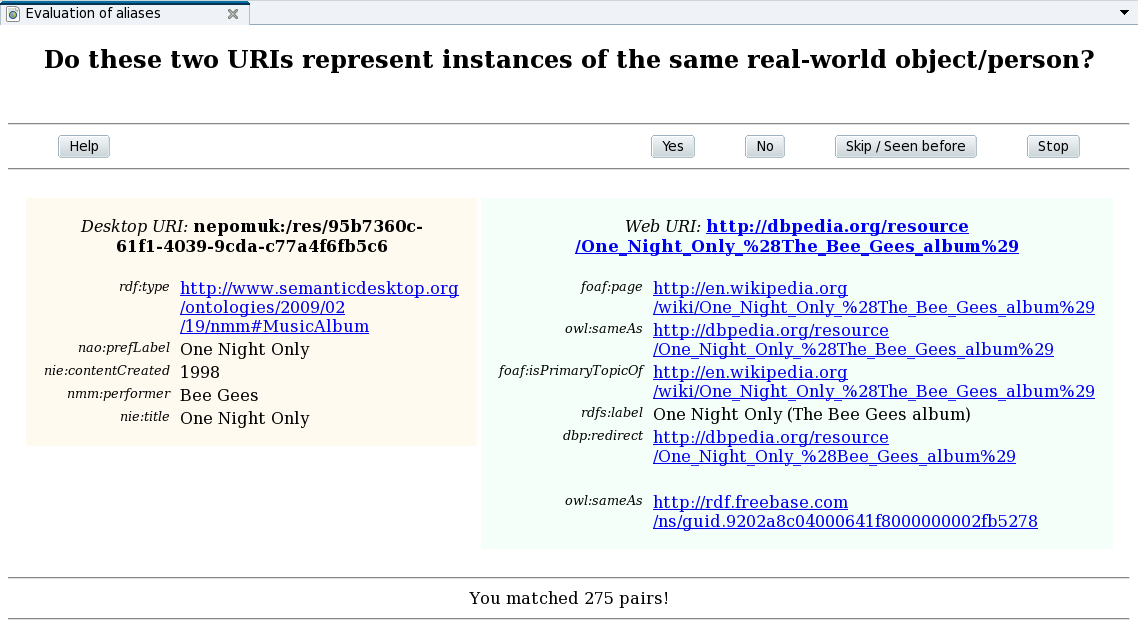
\includegraphics[width=\linewidth]{chapters/core/img/eval_album.png}
\caption{The Web interface of the experiment for collecting relevance judgements.}
\label{fig:onlineexperiment}
\end{figure} 

There were only two decisions possible: \emph{Yes} or \emph{No}, with a \emph{Skip} option, in case of uncertainty. Once a pair was judged or skipped, another one was shown to the participant. The pairs were randomly chosen from the remaining set. To add a gamification element to the experiment, we kept count of the number of pairs judged by each participant, and displayed it on the page. We found that even such a small addition generated ad-hoc competition and made the dull task more interesting.

The results of the experiment show an average agreement and its standard deviation, computed with Fleiss's $\kappa$, of $0.638\pm0.214$, over all three types of entities, suggesting substantial agreement between annotators. Table~\ref{tab:agreementsdwod} shows the Fleiss's $\kappa$ and its standard deviation $\sigma$ per type, as well as the average pairwise percent agreement. We observed that for music albums, there was only moderate agreement between annotators, visibly lower than the average, while for publications it is visibly higher. We believe the difference is caused by the fact that the data about publications is generated and curated by experts in the field --- even more so, as the publications were largely from the domain of Semantic Web --- while the music data comes from much more heterogeneous sources.

\begin{table}
\centering
\ra{1.3}
\begin{tabular}{@{}rcl@{\hs}l@{\hs}l@{}}
\toprule
& \phantom{a} & $\kappa$ & $\sigma$ & Avg  \\ 
\midrule

 All && 0.638 & 0.214 & 92.252 \\

 People && 0.661 & 0.257 & 88.2 \\

 Publications && 0.786 & 0.127 & 98.067  \\

 Albums && 0.442 & 0.233 & 90.523 \\

\bottomrule
\end{tabular}
\caption{Inter-annotator agreement measures}
\label{tab:agreementsdwod}
\end{table}

\subsection{Quantitative Results}

To evaluate the performance of the algorithm, we evaluate each of the matching parameters described in Section \ref{sub:matchingcomp}, activated either separately or using a combination of them, against a baseline which is the matching framework with all the parameters disabled. In the following, the String Matching parameter is denoted by SM, the Weighted Properties by WP and the Multi-Valued Properties by MVP.

We used the \emph{trec\_eval} tool\footnote{\url{http://trec.nist.gov/trec_eval/}} to compute standard information retrieval measures.
The precision at k ($P@k$) with k={1,2,3,4,5}, mean average precision (MAP) and normalised discounted cumulative gain (NDCG) are reported in Table~\ref{tab:agreement-albums} for music albums, Table~\ref{tab:agreement-people} for people and Table~\ref{tab:agreement-publications} for publications. 
We report also the interpolated precision at recall cut-off points when all matching parameters are enabled. The goal for the system is high precision, i.e., achieving a maximum at P@1. Recall is not a target, as it is generally impossible to determine the entire set of correct results available in the Web of Data.

\begin{table}[htb]
\centering
\ra{1.3}
\begin{tabular}{@{}rcl@{\hs}l@{\hs}l@{\hs}l@{\hs}l@{\hs}l@{\hs}l@{}}
\toprule
& \phantom{a} & MAP & NDCG & P@1 & P@2 & P@3 & P@4 & P@5 \\ 
\midrule

 SM WP MVP && 0.2464 & 0.5117 & 1 & 0.625 & 0.4167 & 0.3125 & 0.25 \\ %111

 SM WP && 0.2464 & 0.5117 & 1 & 0.625 & 0.4167 & 0.3125 & 0.25 \\ %110

 SM MVP && 0.2464 & 0.5117 & 1 & 0.625 & 0.4167 & 0.3125 & 0.25 \\ %101

 WP MVP && 0 & 0 & 0 & 0 & 0 & 0 & 0 \\ %011

 SM && 0.2464 & 0.5117 & 1 & 0.625 & 0.4167 & 0.3125 & 0.25 \\ %100

 WP && 0 & 0 & 0 & 0 & 0 & 0 & 0 \\ %010

 MVP && 0 & 0 & 0 & 0 & 0 & 0 & 0 \\ %001

 Baseline && 0 & 0 & 0 & 0 & 0 & 0 & 0 \\ %000

\bottomrule
\end{tabular}
\caption{Evaluation results for albums, when varying configuration parameters.}
\label{tab:agreement-albums}
\end{table}

In Table~\ref{tab:agreement-albums}, we can observe that only the SM parameter is enhancing the results compared to the baseline. The other two parameters do not improve the results at matching certain candidates. Also, in term of MAP and NDCG, the system achieves the lowest performance on the albums corpus. This can be explained by the fact that the Web resources returned by the query module for albums are mostly e-commerce products, which are not defined as a type of interest, and therefore are rejected by the matching module. However, some of the annotators have considered that the corresponding candidates are indeed the same as the album, while some have disagreed --- this is reflected in the agreement measure, as for the albums we have the lowest value for Fleiss's $\kappa$. Whether or not such candidates should have been kept by the system is open to discussion and left for future work.

\begin{table}[htb]
\centering
\ra{1.3}
\begin{tabular}{@{}rcl@{\hs}l@{\hs}l@{\hs}l@{\hs}l@{\hs}l@{\hs}l@{}}
\toprule
& \phantom{a} & MAP & NDCG & P@1 & P@2 & P@3 & P@4 & P@5 \\ 
\midrule

 SM WP MVP && 0.4212 & 0.6354 & 0.9302 & 0.8953 & 0.7597 & 0.6337 & 0.5442 \\ %111

 SM WP && 0.4174 & 0.6321 & 0.9286 & 0.8929 & 0.746 & 0.6131 & 0.5286 \\ %110

 SM MVP && 0.4212 & 0.6354 & 0.9302 & 0.8953 & 0.7597 & 0.6337 & 0.5442 \\ %101

 WP MVP && 0.2916 & 0.5338 & 1 & 0.8243 & 0.6036 & 0.473 & 0.3838 \\ %011

 SM && 0.4212 & 0.6354 & 0.9302 & 0.8953 & 0.7597 & 0.6337 & 0.5442 \\ %100

 WP && 0.2916 & 0.5338 & 1 & 0.8243 & 0.6036 & 0.473 & 0.3838 \\ %010

 MVP && 0.2877 & 0.53 & 1 & 0.8243 & 0.6036 & 0.4662 & 0.3784 \\ %001

 Baseline && 0.2877 & 0.53 & 1 & 0.8243 & 0.6036 & 0.4662 & 0.3784 \\ %000

\bottomrule
\end{tabular}
\caption{Evaluation results for people, when varying configuration parameters.}
\label{tab:agreement-people}
\end{table}

In Table~\ref{tab:agreement-people}, we can observe that the baseline, the WP and the MVP parameters are each able to match good candidates with high precision at P@1, with WP providing slightly better MAP and NDCG. However, the system does not get significant advantage by combining them. The SM parameter alone provides slightly lower precision at P@1 but significantly better MAP and NDCG. By combining the three parameters, the system does not get significant advantage and it seems that using SM prevails. 

\begin{table}[htb]
\centering
\ra{1.3}
\begin{tabular}{@{}rcl@{\hs}l@{\hs}l@{\hs}l@{\hs}l@{\hs}l@{\hs}l@{}}
\toprule
& \phantom{a} & MAP & NDCG & P@1 & P@2 & P@3 & P@4 & P@5 \\ 
\midrule

 SM WP MVP && 0.7773 & 0.8651 & 1 & 0.625 & 0.4167 & 0.3125 & 0.25 \\ %111

 SM WP && 0.8032 & 0.8609 & 0.9062 & 0.5781 & 0.3958 & 0.3047 & 0.2438 \\ %110

 SM MVP && 0.7175 & 0.7986 & 0.9231 & 0.5769 & 0.3846 & 0.2885 & 0.2308 \\ %101

 WP MVP && 1 & 1 & 1 & 0.5 & 0.3333 & 0.25 & 0.2 \\ %011

 SM && 0.7265 & 0.7883 & 0.8235 & 0.5294 & 0.3627 & 0.2868 & 0.2294 \\ %100

 WP && 0.6893 & 0.7347 & 1 & 0.55 & 0.3667 & 0.275 & 0.22 \\ %010

 MVP && 0 & 0 & 0 & 0 & 0 & 0 & 0 \\ %001

 Baseline && 0.7175 & 0.7588 & 1 & 0.5455 & 0.3636 & 0.2727 & 0.2182 \\ %000

\bottomrule
\end{tabular}
\caption{Evaluation results for publications, when varying configuration parameters.}
\label{tab:agreement-publications}
\end{table}

In Table~\ref{tab:agreement-publications}, the baseline provides good results from the start for publications. The system is not able to return any candidates when MVP alone is activated. However, when WP and MVP are combined, the system achieves much better results (in term of MAP and NDCG) than the baseline or than the WP parameter alone. When the system combines SM with the two previous ones, the system achieves a lower MAP and NDCG but an improved precision with a larger cut-off rank. While on the two previous types of entities, the SM parameter seemed to be the most important matching feature, this corpus shows that the WP and MVP are important matching features in certain cases.

\begin{figure}[htb]
 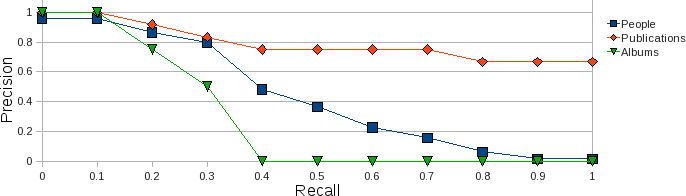
\includegraphics[width=\linewidth]{chapters/core/img/precrecal_wlabels.png}
\caption{Interpolated precision at recall cut-off points.}
\label{fig:precrecall}
\end{figure}

Overall, the results are satisfying for our use cases where high precision prevails over recall. However, given the results shown in Figure~\ref{fig:precrecall}, we can see that the system could be configured to return more than one entity in order to achieve better recall while keeping good precision. It might prove useful to implement a semi-automatic system which presents the top \emph{n} candidates to the user for manual selection.

\subsection{Performance}

To determine the performance, we measured the time spent on each step of the algorithm. We note that these results come from a prototype implementation, still to be subject to technical optimisations. Table~\ref{tab:sdwodtimes} shows the average times overall, and for each resource type separately, when all three parameters (SM, WP, MVP) are active. We find only small variations in the measurements when the parameter values are changed. We do not consider the time spent on retrieving data from Sindice, as this depends on external factors, like network speed and server availability. 

\begin{table}[htb]
\centering
\ra{1.3}
\begin{tabular}{@{}rcr@{\hs}r@{\hs}r@{\hs}r@{}}
\toprule
& \phantom{a} & Overall & People & Publications & Albums \\ 
\midrule

 Pair total && 375.04 & 52.19 & 977.87 & 53.18 \\

 Types check && 0.23 & 0.26 & 0.21 & 0.23 \\

 Per property check && 6.66 & 0.92 & 13.2 & 22.06 \\

 All properties && 2026.22 & 7.17 & 5478.87 & 1963.88 \\

\bottomrule
\end{tabular}
\caption{Time performance (milliseconds).}
\label{tab:sdwodtimes}
\end{table}

The checking of types is the only value that on average does not depend on the type of resource, as it must be performed for all pairs. The time spent in average per property check is low, but it varies by type, and by the complexity of the properties (e.g. it takes longer if several resources in the graph must be traversed, for long property paths like the name of the artist of an album). The ``All properties'' row shows the average time required for checking all the properties of an entity, and the computation of the final score\footnote{The ``All properties'' row has values higher that the ``Pair total'' row because the average time is computed only for those pairs that passed the type check, thus fewer, but with longer computation times.}. These values depend on the type of resources as well, and on the complexity of the resource graph. We found that longer times correspond to very big graphs for online entities, which must be loaded for checking even if in most cases are not found to represent valid 
candidates\footnote{e.g., the graph for \url{http://webconf.rkbexplorer.com/models/iswc-aswc-2007-complete.
rdf}}.


\section{Discussion}

The scope of the system presented here is limited to finding Web of Data aliases for desktop resources. We leave the use of the aliases found to future work, but the use cases include personalised desktop services like those described in Section~\ref{sec:sdwodintro} and enhancement of desktop information from online sources like the one described in \cite{Groza2009}. We plan to develop a semi-automatic service that retrieves information from the Web aliases and updates the local resources, while saving provenance information for the imported data and allowing synchronisation when the Web data changes.

Existing Web applications already provide similar services via specific APIs (e.g., last.fm). However this is not the goal of our work. Instead, we wish to leverage information across all public information sources accessible on the Web of Data. In addition, such third-party APIs are seen as an additional information sources on the Web, and are supported by our system.

Within the system, we make use of existing semantic technologies, including semantic search engines such as Sindice. In the process of determining the aliases we focus on selecting the most appropriate URI from the list of candidates returned by the search engine. In this case, the issue of which data sources to trust is left to the search engine, which usually employs advanced techniques~\cite{Delbru2010} for making the decision. This is however not a requirement we impose on the users, who can choose to query other trusted data sources suitable for their use case.

The system we presented is automatic, as no user interaction is required for it to work. Once set up it will find and save aliases to desktop resources. 
Although the mappings were created manually, they are part of the system and do not need to be modified by end users. 
Power users can however tweak the settings to fit their specific needs by enabling or disabling modules, changing threshold values or modifying mappings.
While new mappings can only be created manually, expert users can take advantage of the openness resulting from the use of SPARQL-based search mechanism and update the mappings as they need, or create new ones. We envision for the future, a way of allowing power users to publish their own mappings and let other users install new mappings in a way similar to installing add-ons to Web browsers.


\section{Conclusion}

In this chapter, we presented a framework to automatically link entities from the Semantic Desktop to the Web of Data. This is the logical next step after the creation of semantic data on the desktop, presented in the previous chapter.

The framework uses existing technologies such as semantic search engines and public SPARQL endpoints for retrieving a set of candidates. Each candidate is then evaluated more precisely based on a collection of matching components using string matching, heuristics and rule-based mechanisms. We evaluate the system qualitatively, using real-world data retrieved from a Nepomuk-KDE Semantic Desktop and the Sindice search engine. The evaluation is based on relevance judgements from a group of experts. We show that the system in its current form provides satisfactory results in term of precision for automatic linking of entities.

Once the two networks of linked data are connected, we can build semantic applications and services using personal data from the desktop and enriched with information from the Web of Data. In the next chapter we present one such application.


\chapter{Transforming Semantic Notes into Semantic Blog Posts}
\label{ch:semblogging}

\begin{flushright}
 \textit{Based on ``Linking Semantic Personal Notes'' \cite{Dragan2010a}\\published at the Workshop on Knowledge Injection into and Extraction from Linked Data (KIELD~2010~co-located~with~EKAW~2010)}
\end{flushright}

In the previous two chapters we showed how Semantic Web technologies are available both on the desktop and of course on the Web, and how the two networks of linked data can be connected. SemNotes, a semantic note-taking tool for the Semantic Desktop, described in Chapter \ref{ch:semnotes}, shows how new data can be created and seamlessly integrated with existing semantic information from the desktop. Chapter \ref{ch:sdwod} describes an algorithm for automatically connecting desktop resources to their Web aliases, bridging the gap between the desktop and the Web in regards of semantic data, opening up the possibility of augmenting desktop data and building personalised desktop services. 

In this chapter we present a use case, and a proof of concept system which builds on our previous work in order to support easy publishing and sharing of semantic personal notes taken with SemNotes as Linked Data.
Our approach can be used to publish any kind of information from the desktop to the Web, enabling integration of small chunks of personal knowledge into the Web of Data.
This use case illustrates a solution to the second research question \textbf{Q 2.} from Section \ref{sub:question}, \emph{How to expand the scope of the Semantic Desktop into the realm of the Web of Data, to enhance the user experience and benefit?}, more specifically, to the second and third sub-questions \textbf{Q 2.2.} --- \emph{How to use the Web information found related to a desktop resource?}, and \textbf{Q 2.3.} --- \emph{How to make desktop data available online safely?}

\section{Introduction}
\label{sec:introduction}

Semantic Web technologies are deployed in various domains and applications, both on the desktop and on the Web.
While these two domains share compatible representation models (RDF(S)/OWL), there is still a gap between data from the Web and the desktop. We showed in the previous chapter how finding Web aliases for Semantic Desktop resources enables us to bridge this gap. This solution is however unidirectional --- it only solves connection from the desktop to the Web, and not the reverse, from the Web to the desktop. It can be argued that accessing desktop information from the Web is not necessary, or not safe, or that the risks exceed the benefits. However, sharing desktop information online has many possible use cases, and does not necessarily involve making private information public. 

One such use case of sharing desktop information and realising better integration of personal data with online data, is described in this chapter. We present an approach for publishing personal notes from the desktop (using SemNotes and Semantic Desktop technologies) to the Web of Data (using the Linked Data principles). Our goal is to publish this data online without losing the personal context established on the desktop through the links from the notes and the related desktop resources.
Our approach consists of two main steps: 
\begin{enumerate}
 \item preparing the desktop data for sharing, 
 \item publishing it online. 
\end{enumerate}
In addition, it requires two prerequisite steps, which are supported by previous work: 
\begin{itemize} 
 \item the note-taking process and annotation of the note (adding the context) which was presented in Chapter \ref{ch:semnotes}, and 
 \item the identification of Web URIs which represent the same real-world thing as the desktop resources that belong to the context of a note, which was presented in Chapter \ref{ch:sdwod}. 
\end{itemize}

Our contribution consists of the process for publishing personal information from the desktop to the Web following the Linked Data principles \cite{BernersLee2006}, and a system implementation that allows sharing of semantic personal notes as semantic blog posts, interlinked with existing information from the Web of Data. 
The publication process must follow the Linked Data principles, while at the same time protecting sensitive private data from being shared unwillingly, and maintaining the meaningful relations in the process.


The semantic notes taken with SemNotes constitute the personal information that we want to publish as Linked Data. They are semantically linked to local resources mentioned in their content, like people, projects or other notes. If the notes were directly published online, the relations that enrich them would be lost and the links they contain would be broken, because they point to local URIs not available outside of the desktop. The same objects often exist within the Web of Data, therefore the note links to them can be recreated in the publishing process. Before the note is published, our system searches for existing public Web aliases for the local resources. They are then used to substitute the local private data referenced in the text --- the links are changed to point to the Web resource. In this way, the published links are valid, the meaning of the link is preserved (as referring to the same entity) and the private information is protected. The system then publishes the notes online as blog posts 
taking care of the transformations required from desktop ontologies to Web ones, according to the mappings devised in Chapter \ref{ch:sdwod}.

In line with the two-step process mentioned above, our system has two modules, one working on the desktop and the second one online. First, the desktop part handles the preparation of the notes for publishing, using the Web aliases identified by the service described in the previous chapter, substituting them for the local ones, as well as the transformation required from desktop ontologies to Web ones. This module is invisible to the user, except for the \emph{Publish} button shown in the user interface of SemNotes. Then, the Web part publishes the transformed notes as Linked Data in accordance with the Linked Data publishing principles.

The solutions provided by most existing systems fall into two categories: \begin{inparaenum}[(i)] \item desktop applications that involve publishing the actual local resource information together with the note, or \item online applications that do not have access to desktop data relevant to the user. \end{inparaenum} The first category, represented by tools like SemiBlog \cite{Moeller2005} or SemBlog \cite{Takeda2005}, is not optimal when dealing with resources that contain sensitive private information. Services like Zemanta\footnote{\url{http://www.zemanta.com}}, from the second category, have access to various online resources, but not to the personal context of the user.
Also they miss the personal touch of desktop-based applications.


\section{From Note-Taking to Weblogging}
\label{sec:reqsemblog}

Two characteristics of blog posts which are relevant to this use case are: 
\begin{itemize}
 \item their topics are of interest to the author and thus are very likely to have references to things also present on the desktop (e.g. people, events); 
 \item the context consists of the references made in their content, such as places, projects, or other blog posts.
\end{itemize}

However, not all blog posts start by being a blog post. Some are just ideas or impressions jotted down for later, in one's preferred desktop note-taking application. Nevertheless, some of these notes do become posts after polishing and refining, especially as some notes might require further investigation before they can be published (e.g. when writing on a technical subject). Examples include notes taken at presentations, ideas on topics of interest written down at times when blogging is not possible (attending a meeting or lack of Internet connection).

Tools from the Semantic Desktop, like SemNotes, provide means to enhance these notes locally, by interlinking them with other desktop data --- the contacts in the address book, the events from the calendar application, the projects worked on, the music listened to. 
For example, a note about an upcoming concert can be linked to the performing artist which is in turn linked to the music files of that artist and pictures from earlier shows stored in a desktop photo application.
Such annotations give context to the note and should be preserved when the note is published as a blog post on the Web, since it enables serendipitous browsing and information discovery, through the relevant additional links they contain.

Currently, personal notes, even the ones semantically enriched using Semantic Desktop applications, must be published as blog posts by being manually copied into a blogging tool.
In this way, any additional semantic information available on the desktop is lost or, if copied, leads to broken references as they point to the local resources which are not accessible outside of the desktop.
The note-taking to publishing process is sometimes cut short by using the drafting functionality offered by some systems like WordPress or Blogger, so that users can directly take the notes in the blogging tool, usually online, thus replacing the desktop note-taking application completely. However, using online tools deprives the user from having the personal context added to the blog post, since desktop information cannot be easily integrated in Web-based services.

In order to enable a better transition from personal notes to blog posts, or simply to Web-based information available to others (for example, meeting notes published in a company intranet or lecture notes shared between students of the same class), we defined a list of requirements that a system for publishing semantic personal data online should fulfil:
\begin{description}
 \item[R1.] Publish the complete desktop data on the Web without losing any relevant information, including metadata and context (e.g. tags, relations, identifiers);
 \item[R2.] Protect any machine readable and private data that might be unwillingly included in the context being transferred\footnote{The protected data does not include the actual text to be shared as it is a conscious decision to publish it, taken explicitly by the user};
 \item[R3.] Publish the note according to the Linked Data principles and describe it using popular ontologies; 
 \item[R4.] Enable object-centred sociality by establishing connections between data published by different users.
\end{description}


\section{Overview of the Process and Prerequisite Steps}
\label{sec:sembloggingapproach}

We propose an approach that enables the publishing and sharing of personal notes by extending the functionality provided by SemNotes, and by using the Web of Data aliases found for desktop resources. The process consists of two steps: 
\begin{enumerate} 
 \item transformation, and 
 \item publication. 
\end{enumerate}
In the first step, the note is transformed locally for publication, and private local data is replaced with public references.
In the second step, the transformed note is published online.

The system requires a dedicated server, where the resources referenced and the tags assigned are shared between the notes of all users, to add a social aspect. Also, rather than trying to determine which of the many possible Web aliases found for a desktop resource is authoritative, we let the server create equivalent public resources and connect all the aliases to them. We also used the server for publishing the notes, although this can be replaced by any other blogging platform.

The first prerequisite step --- note-taking and annotation of the note with the relevant desktop resources --- must be performed before any actual sharing of notes can be done. The annotation is done semi-automatically and is an existing feature in SemNotes. 

The second prerequisite step consists in finding Web resource for each of the desktop entity linked to the note that is about to be published. This step is executed by a desktop service which implements the two-part algorithm detailed in the previous chapter, the blocking pass using Sindice to retrieve possible candidates and filtering the list by the score returned by the matching algorithm. The local service has access to, and uses all the information available on the desktop about a resource to identify only exact matches for it. The aliases which are found for the desktop resources are saved by creating a \verb|pimo:hasOtherRepresentation| link in the local repository between the desktop resource and the Web one.


\section{System Implementation Details}
\label{sec:sembloggingsystem}

Based on the process described above, the system is divided between its local part and its remote part, as shown in Figure \ref{fig:semblogsystem}. The local part handles local \emph{private} data, while the remote one handles online \emph{public} data. 
\begin{figure}[htb]
  \begin{center}
    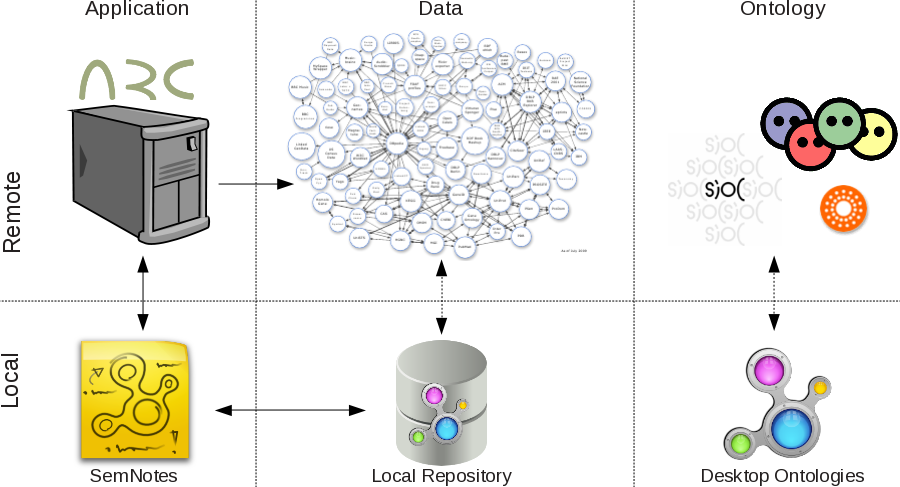
\includegraphics[width=0.8\linewidth]{chapters/core/img/system}
    \caption{Overview of the semantic publishing system.}
    \label{fig:semblogsystem}
  \end{center}
\end{figure}
The separation between them extends over three layers: ontology, data and application.
On the \emph{ontology} layer, the NEPOMUK desktop ontologies are used locally, while popular Web vocabularies are used on the server-side. These ontologies are used to describe the \emph{data} exchanged between the applications. Desktop data is stored in the local NEPOMUK repository, while Web data is distributed. Finally, on the \emph{application} layer, the local component is an extension to SemNotes that provides publishing functionality for notes, and the remote component is a server that hosts and publishes online the notes received.

The first step of the process --- transformation --- is executed on the local side, by an extension of the SemNotes application. Then, the publication step is done by the server, which receives information from the desktop and publishes the note, as we will describe next. The two application components, the communication between them, and the data translation process are described in detail below.

\subsection{Ontologies}

Although both the Semantic Desktop and the Semantic Web use the same representation languages, i.e. RDF(S)/OWL, they use different vocabularies to describe their data. This vocabulary gap makes data integration difficult.

The NEPOMUK project defines a set of desktop ontologies to describe its data.
SemNotes uses these ontologies to represents personal notes as instances of \verb|pimo:Note| and are linked to the \verb|pimo:Thing|s they mention by the relation \verb|pimo:isRelated|. 

When a desktop resource is found to represent the same real world entity as a Web resource, the relation is stored on the desktop as \verb|pimo:hasOtherRepresentation|. This property is recommended by the PIMO specification as desktop equivalent to the \verb|owl:sameAs| relation, although without the formal semantics that the latter provides. We also use the property \verb|pimo:hasOtherRepresentation| to store the remote URL of a note when it is published. If the note changes on the desktop after publication, the property is replaced with \verb|pimo:hasDeprecatedRepresentation|.

While well-suited to represent desktop information, these ontologies are not used, so far, on the Web. However, numerous vocabularies have emerged for describing semantic data published online. Such ontologies have now been widely adopted and are recommended as best practices when publishing data on the Web \cite{Bizer2007}. 

Consequently, while representing similar objects, the two sets of vocabularies must be aligned so that on the one hand, desktop information can be moved to the Web and understood by usual Semantic Web applications that rely on the aforementioned vocabularies, and on the other hand, Web information could be understood and imported by Semantic Desktop applications. In order to enable interoperability between the desktop and the Web, we defined mappings between the sets of ontologies. The mappings create appropriate subclasses or subproperties of the relevant concepts from the chosen vocabularies.

SIOC is probably the most widely used vocabulary for interlinking social media within the Web of Data.
There are already many tools for creating and using SIOC data \cite{Bojars2008}.
This is why we chose to represent the \verb|pimo:Note|s as \verb|sioc:Post|s when they are published online with our system. The rest of the desktop resources are also transformed into concepts from the vocabularies listed above (see Table \ref{tab:classmappings}), the mappings being published at \url{http://rdfs.org/sioc/nepomuk}.
\begin{table}[htb]
\centering
\ra{1.3}
\begin{tabular}{@{}rcl@{}}
\toprule
Class && Subclass of \\ 
\midrule

\verb|pimo:Note| && \verb|sioc:Post| \\

\verb|nao:Tag| && \verb|sioct:Tag| \\

\verb|pimo:Person| && \verb|foaf:Person| \\

\verb|pimo:Project| && \verb|doap:Project| \\

\verb|pimo:Event| && \verb|ical:Vevent| \\

\bottomrule
\end{tabular}
\caption{Sample of the mapping between classes.}
\label{tab:classmappings}
\end{table}
The note's properties, like title, creation and last modification time, are translated to the appropriate Dublin Core properties: \verb|dcterm:created|, \verb|dcterms:modified| and \verb|dcterms:title|. The tags associated locally with the notes are transformed into \verb|sioct:Tag|s associated with the published post using the \verb|sioc:topic| property. Table \ref{tab:propmappings} lists the proposed mappings for properties\footnote{Although \texttt{nao:lastModified} and \texttt{dcterms:modified} do not have the same semantics, defining subproperty relations between them is acceptable.}.

\begin{table}[htb]
\centering
\ra{1.3}
\begin{tabular}{@{}rcl@{}}
\toprule
Property && Subproperty of \\ 
\midrule

\verb|nao:prefLabel| && \verb|rdfs:label| \\

\verb|nao:created| && \verb|dcterms:created| \\

\verb|nao:lastModified| && \verb|dcterms:modified| \\

\verb|nao:hasTag| && \verb|sioc:topic| \\

\verb|pimo:isRelated| && \verb|sioc:related_to| \\

\bottomrule
\end{tabular}
\caption{Sample of the mapping between properties.}
\label{tab:propmappings}
\end{table}


\subsection{Server Schema}

In order to publish the resources with a consistent URI scheme, we defined patterns for naming the objects published from the desktop on the Web. In the schema definition, we apply several Linked Data patterns described in \cite{Dodds2010LDPBook}: 
\begin{itemize} 
 \item patterned URIs --- for all the entities, to make them more human readable; 
 \item proxy URIs --- for the server URIs, to group multiple Web aliases;
 \item equivalence links --- for the resources related to the notes, to unify various sources; 
 \item natural keys --- in the tag URIs. 
\end{itemize}

For each note the server generates a new unique identifier \verb|id| which is used to create the note's URI in the form: \verb|http://notes.server/note/id|.

According to the proxy URIs identifier creation pattern, we generate new URIs for the resources related to the notes. This ensures that the publishing process is consistent and avoids having to choose among several Web aliases a resource could have. Like the notes, each resource has a unique identifier on the server, which is used to create the resource URI according to the following format: \verb|http://notes.server/resource/id|. Resources are shared by all the notes that link to them, which increases the interlinking and the consistency of the data. For each resource, the server keeps internally a list of Web aliases using \verb|owl:sameAs| links.

Tags are considered a particular type of resources, and are also shared on the server. The specific format for the URI: \verb|http://notes.server/tag/label|, differentiates them from regular resources. The label of the tag acts as a unique identifier, and is case sensitive. They are created on the fly, and are persisted when they are used for the first time.


\subsection{Transformation of the Notes for Sharing}

The first step of the process consists of preparing the note for publishing. In this phase all the relevant information about the note is included in the content, specifically the title, creation and last modification time, the tags and the referenced resources. This transformation is necessary, so that less information, specifically only the HTML content of the note is sent to the server, and not the entire RDF graph describing the note. Although the content is already stored as HTML, to include all the metadata about the note, it has to be enriched with RDFa before being posted to the server.

The preparation step is done on the desktop side, by the added extension to SemNotes. 
To include the referenced resources in RDFa, we need to know their server URIs. Therefore the application needs to communicate with the server to retrieve several URIs: 
\begin{itemize}
 \item the URI for the new note to be published, and 
 \item the server URI for each resource referenced by the note. 
\end{itemize}

In case the note has already been published, the user can overwrite the old post (on the Web) or create a new one. Depending on this choice, a new URI is requested from the server, or the existing one is used (that was saved in the local repository when the note was previously published). 

The referenced resources are shared by all the published notes, therefore the server must create the URI for a resource only if it has not been created before. To decide whether a local resource already has a server URI created, the list of Web aliases found for it on the desktop in the second prerequisite step of the process, is sent to the server (see JSON data in Listing \ref{lst:messagetoserver}). If a resource with a matching type and an overlapping list of aliases exists, the server reuses it, otherwise it creates a new one and saves the information about it in its own RDF repository. On the server, the URI aliases are saved as \verb|owl:sameAs| as it is customary for Linked Data. The server URIs for the note and the resources are also stored on the desktop for reuse, as \verb|pimo:hasOtherRepresentation|.
\lstset{
	caption={JSON formatted message sent to the server.}, 
	label=lst:messagetoserver,
	language=js
}
\setlength\parindent{0in}
\begin{minipage}[t]{\linewidth}
\begin{lstlisting}
{
   "id" : "",
   "resources": [
   {
      "id": "nepomuk:/res/bfcdcd1a-4898-492f-940b-4cc4c67799a7",
      "type": "mo:MusicArtist",
      "uris": [
         "http://dbpedia.org/resource/Scorpions_(band)",
         "http://musicbrainz.org/artist/c3cceeed-3332-4cf0-8c4c-bbde425147b6"
      ]
   }
   ]
}
\end{lstlisting}
\end{minipage}
\setlength\parindent{0.21in}

\lstset{
	caption={Server reply with the server URIs for the resource aliases sent.}, 
	label=lst:serverreply,
	language=js
}
\setlength\parindent{0in}
\begin{minipage}[t]{\linewidth}
\begin{lstlisting}
{
   "note":{
      "uri":"http://notes.server/note/4baccab834e20",
      "resources":[
         {
            "local":"nepomuk:/res/bfcdcd1a-4898-492f-940b-4cc4c67799a7",
            "uri":"http://notes.server/resource/4bacca84ca8bb"
         }
      ]
   }
}
\end{lstlisting}
\end{minipage}
\setlength\parindent{0.21in}

In the case when no Web aliases are found for a desktop resource that is related to a note, and thus the list of aliases sent to the server is empty, a new resource is created on the server with the specified type, but without any information attached to it. The server URI is saved on the desktop as \verb|pimo:hasOtherRepresentation| of the resource, and will be available for reuse when other notes related to the same object are published by the same user. However, this resource will not be shared between notes published by different users. If at a later stage a Web alias is found for the desktop resource, it will be added to the resource already created on the server, thus enabling it to be linked to by multiple users.

The communication between SemNotes and the server is done with a single REST call, in order to minimise network delays. The reply contains the newly created URI for the note, if one was required, as well as a list of server URIs for the resources (see JSON data in Listing \ref{lst:serverreply}). The communication between the desktop side and the server is shown in Figure \ref{fig:semblogsequencediag}. 

Using the information received from the server, the note content is enriched with RDFa. The metadata about the note, like type, creation and last modification times and the tags, is added in \verb|meta| tags in the \verb|head| of the HTML page. RDFa is added to the \verb|title| tag and in the \verb|body|, to the links. Listing \ref{lst:rdfa} shows the content of a note prepared for publishing.

\begin{figure}[htb]
  \begin{center}
    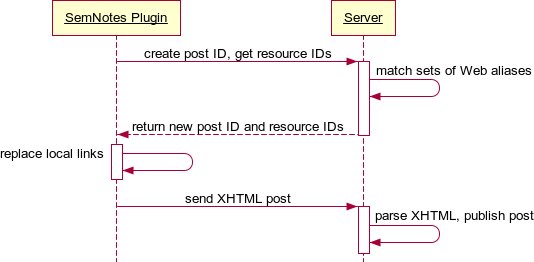
\includegraphics[width=0.85\linewidth]{chapters/core/img/sequencediagram}
    \caption{Sequence diagram for the communication with the server.}
    \label{fig:semblogsequencediag}
  \end{center}
\end{figure}

\lstset{
	caption={RDFa-annotated XHTML content of note.}, 
	label=lst:rdfa,
	language=htmlrdfa
}
\setlength\parindent{0in}
\begin{minipage}[t]{\linewidth}
\begin{lstlisting}
<!DOCTYPE html PUBLIC '-//W3C//DTD XHTML RDFa 1.0//EN' 
                      'http://www.w3.org/MarkUp/DTD/xhtml-rdfa-1.dtd'>
<html about="http://notes.server/note/4baccab834e20">
    <head>
        <meta content="sioc:Post" property="rdf:type"/>
        <meta rel="sioc:topic" href="http://notes.server/tag/concert"/>
        <title property="dc:title">concert sunday</title>
    </head>
    <body>
        <a rel="sioc:is_related"
             href="http://notes.server/resource/4bacca84ca8bb">scorpions</a> concert on sunday was great ...
    </body>
</html>
\end{lstlisting}
\end{minipage}
\setlength\parindent{0.21in}


\subsection{Publication Step}

After the preparation step, which takes place on the desktop side, the RDFa enriched content is sent to the server via another REST call. The publication step of the process only handles public data. When the content is received it is parsed and the server extracts the contained RDF triples and stores them in its repository. The content (as it is received) is also stored.

The server implementation uses ARC2\footnote{\url{http://arc.semsol.org}}, as it provides out of the box RDFa parsing and an RDF repository. It is easily deployable due its minimal setup requirements (a PHP enabled Web server and a MySQL database), thus making our system easily deployable as well.

All server URIs are dereferenceable, as required by the Linked Data principles. For notes, the URI redirects to the RDFa annotated HTML page containing the note itself (as shown in Figure \ref{fig:views} (i)), the URI of the note being the URL of this page. For the linked resources, the URI is also dereferenceable and provides RDFa information about itself, linking to the known existing Web aliases of the same resource. The description also includes a list of backlinks to all the notes that reference the resource (see Figure \ref{fig:views} (ii)). The page for a tag will contain backlinks to all the notes tagged with it.

The RDFa annotated page for the note is generated on the user's desktop by the SemNotes plugin, as we have seen in the previous step, while the page describing each resource and tag is generated on the fly, by the server, when the URI is requested.

\begin{figure}[tb]
\begin{minipage}[b]{0.49\linewidth}
\begin{flushleft}
    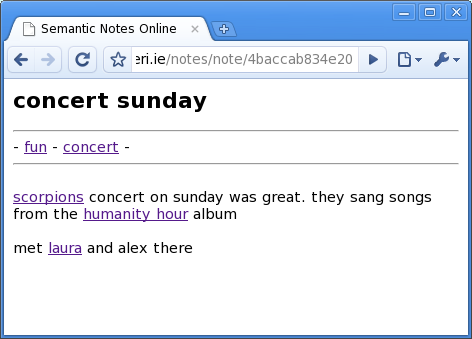
\includegraphics[width=0.97\linewidth]{chapters/core/img/noteview}
\end{flushleft}
\end{minipage}
\begin{minipage}[b]{0.49\linewidth}
\begin{flushright}
    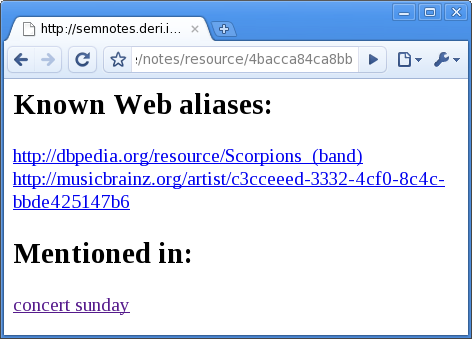
\includegraphics[width=0.97\linewidth]{chapters/core/img/resourceview}
\end{flushright}
\end{minipage}
\caption{Online view of a note (i) and a resource (ii).}
\label{fig:views}
\end{figure}


\section{Conformance with the Initial Requirements}
\label{sec:evaluationsemblog}

When establishing the specifications of the framework, we identified four main requirements (Section \ref{sec:reqsemblog}).
Our proposed implementation conforms with them as follows.

\emph{\textbf{R1}: Publish the complete desktop data on the Web without losing any relevant information, including metadata and context (e.g. tags, relations, identifiers).}\\
By translating existing desktop data surrounding the note to RDF and putting it online, available as RDFa, the entire information available on the desktop side is made available on the Web for further reuse.
In addition, all information from the original note-taking tool, including title, tags, etc. is publicly made available on the Web.

\emph{\textbf{R2}: Protect any machine readable and private data that might be unwillingly included in the context being transferred;.}\\
By replacing the private desktop data with equivalent public Web data, we protect the former. On the desktop there is a lot of private information stored about resources, like the email address or telephone number for people, or the list of attendees of an event. When the person or event is linked to a note that is afterwards published online, such private information is not exported, because the reference to the local resource is replaced by a reference to already public Web data representing the same thing. In this manner, the context of the note being published is preserved, but the private details are not exposed.

\emph{\textbf{R3}: Publish the note according to the Linked Data principles and describe it using popular ontologies.}\\
Our system publishes notes on the Web using the Linked Data principles. Each note and connected resource, has its own URI, which is made dereferenceable, while distinguishing information resources and non-information resources.
In addition, while original desktop data is provided using ``desktop ontologies'', the published information is made available using FOAF, SIOC, Dublin Core, etc. and the mappings have been validated through Vapour\footnote{\url{http://vapour.sourceforge.net/}}.

\emph{\textbf{R4}: Enable object-centred sociality by establishing connections between data published by different users.}\\
Since resources and tags are shared between users, notes can be browsed serendipitously through shared connections, or tags. 
This enables ``object-centred sociality'' \cite{KnorrCetina1997}, since people can interact around these shared tags and topics, such as projects or people that they have in common.
Depending on the destination of the publishing process, there is the possibility of having private notes, yet still accessible online by registered users only.


\section{Related Work}
\label{sec:relatedworksemblog}

Semantic blogging was introduced by \cite{Cayzer2003}, and since then has received much interest. Later \cite{Karger2004} described semantic blogging in the context of the Semantic Web with Haystack. So far, existing systems for semantic blogging fall into two categories: 
\begin{itemize}
 \item desktop applications that involve publishing the actual local resource information together with the blog post, or
 \item online applications that do not have access to desktop data relevant to the user. 
\end{itemize}

The tools in the first category, like SemBlog \cite{Takeda2005} and SemiBlog \cite{Moeller2005}, have the advantage that users have better access to the relevant data from the desktop. However, both tools require that the resources that contain sensitive private information are published together with the blog posts, which might lead to privacy issues. The SemBlog project allows users to add data from personal ontologies to their blogs. SemiBlog allows integration of personal data in the posts by drag and drop from various desktop applications like the address book. SemBlog and SemiBlog are used for exchange of personal information in the blog posts, which differs from our approach of using already published Web data as to protect the privacy of the personal information. SemiBlog's process implies manually adding the metadata, while our approach relies on automatic export. Both tools comply with our first requirement, but not with the last three.

Online services like BlogAccord \cite{Cayzer2006} for music information, and Zemanta\footnote{\url{http://www.zemanta.com}} blogging assistant, belong to the second category. They have access to various online resources to create the context of a blog post and enhance the blogging experience, but they do not use the personal context of the user.



\section{Conclusion}

In this chapter we presented an approach for publishing semantic information from the desktop as Linked Data on the Web. The approach is realised by a system which takes semantic notes from the desktop and makes them part of the Web of Data, as semantic blog posts. The goal of the system is to provide a way for publishing and sharing complete information by preserving the personal context of the notes without compromising privacy. While the use case presented is focused on notes and semantic blogging, the same approach can be applied to publishing of any interlinked information. 

We defined a publishing process that comprises of two steps:
\begin{enumerate}
 \item preparation --- the note is transformed into a SIOC-based Web representation; and
 \item publication and sharing --- the note is published online following the Linked Data principles.
\end{enumerate}

In addition, we provided an implementation of the process, and tested it against a set of requirements regarding publishing personal content from the desktop to the Web as Linked Data.

While we do not authentication issues in this current release, we are considering SW-compliant systems such as FOAF+SSL \cite{Story2009} for future versions of the system.
We also plan to develop additional integration modules for publishing platforms, e.g. Drupal, WordPress, and to investigate approaches for authentication and notification tailored towards the people mentioned in the published data.


\chapter{Additional Extensions and Applications}
\label{ch:mischelperapps}

In this chapter we describe several applications developed in our SmILE\footnote{\url{http://smile.deri.ie}} group at DERI, and to which we contributed. They are extensions to the work presented in the preceding pages, providing or serving as test use cases and validation scenarios.

We start with a list of extensions to SemNotes' functionality, which employ Natural Language Processing techniques. They focus on specific use cases of note-taking, like ontology engineering, meeting minutes or status reports; as well as text analytics tailored to short text.

The work presented in Chapter \ref{ch:sdwod} was initially motivated by the increasingly difficult task of managing publications on the desktop and on the Web, and the need of connecting the information available in both worlds. \emph{Sclippy} is a tool created to avail of the rich information available on the Web about publications, and bring it to the user's desktop. 
The algorithm described in Chapter \ref{ch:sdwod} is a generalisation of the algorithms used in Sclippy\footnote{\url{http://smile.deri.ie/projects/sclippy}}, extending the scope from publications to any type of desktop resources.

We continue by presenting Konduit, a desktop-based platform for visual scripting with RDF data. Based on the idea of the Semantic Desktop, non-technical users can create, manipulate and mash-up RDF data with Konduit, and thus generate simple applications or workflows, which are aimed to simplify their everyday work by automating repetitive tasks. The platform allows to combine data from both the Web and the desktop and integrate it with existing desktop functionality.

\section{Natural Language Extensions for SemNotes}
\label{sec:nlpsemnotes}

During its development phases, SemNotes has served as a sandbox environment and testing bench for several technologies and prototypes developed within our group. Three of the most notable extensions are related to Natural Language Processing (NLP) of the notes, to add functionality. These include: 
\begin{itemize}
 \item a text analytics extension for keyphrase extraction \cite{Schutz2008}
 \item two controlled language extensions for semantic annotation of meeting minutes and status reports \cite{Davis2008,Davis2009}
\end{itemize}

\subsection{Keyphrase Extraction}

Tagging is one of the most used basic features offered by Nepomuk-KDE and by SemNotes. Tags are important for categorisation and organisation of resources, especially for personal notes. Tagging requires users to make a decision on what is relevant about the resource being tagged and how they might reuse the annotation in the future --- i.e. is the tag expressive enough to be later user for filtering the information and finding the required resource. To support users in their choice of tags, and partially automate it, we collaborated on a keyphrase extraction extension to SemNotes. It is based on the TextAnalytics service developed by \cite{Schutz2008}. 

Keyphrase extraction is just one of the NLP functionalities provided by the Text\-Analytics desktop service, alongside information extraction and speech act detection. The service can be accessed by all desktop applications and is available also as an Eclipse plugin for the Java implementation of Nepomuk.

Standard information extraction tools usually extract information which is already known --- like detecting resources in the text. This is the norm in SemNotes as well, where only known existing desktop resources are suggested as annotations of notes, even when other resources might be referred to, but are unknown to the system. The TextAnalytics service is different and complementary, by extracting terms and instances from text, which are not already known to the system. The new terms can become new desktop resources, once identified.

\begin{figure}[tb]
 \centering
 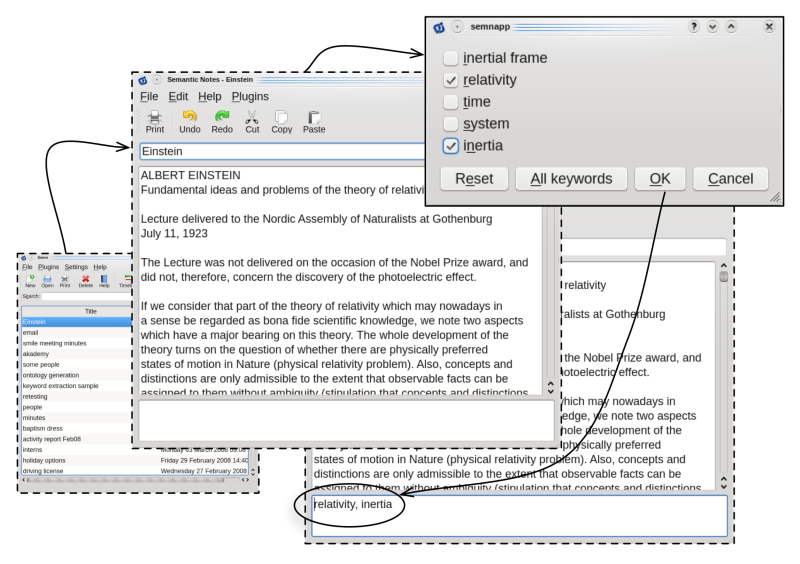
\includegraphics[width=\linewidth]{chapters/core/img/keywordextraction}
 \caption{User interface to keyphrase extraction in SemNotes.}
 \label{fig:keywordextraction}
\end{figure}

We have developed an extension to SemNotes, which uses the service to extract keyphrases from the text of the personal notes and suggest them to the user as tags. The text of personal notes can be small, thus adding difficulty to the extraction task. \cite{Schutz2008} details the way this challenge is tackled in the service. In SemNotes, the service can be called through the menu, and once the note is parsed the relevant terms found are presented to the user as tag suggestions. Figure \ref{fig:keywordextraction}, taken from \cite{Schutz2008}, shows a screenshot of the interface in an older version of SemNotes. If the user accepts any of the suggestions, they become tag resources and are stored in Nepomuk in the usual way.

\subsection{Controlled Language Extensions}

Controlled Natural Languages are well-defined subsets of a natural language with a restricted grammar and lexicon \cite{Schwitter2005}, in order to reduce ambiguity and complexity. In his Ph.D. thesis \cite{Davis2012PhD}, researches the use of Controlled Languages for ontology engineering and semantic annotation. We used SemNotes for prototype testing of both directions, while also providing a feasible use case for the services.

SemNotes, as a note-taking application, is well suited for Controlled Language use, since the main type of input from the users is textual. As a Semantic Desktop application it is also particularly well suited to ontology engineering due to the direct access provided by the framework to the underlying ontologies and desktop resources. As an annotation tool it is also a good testing ground for the semantic annotation using Controlled Language.

\subsubsection{Round Trip Ontology Authoring}

Controlled Natural Language proved efficient for creating ontologies in a user friendly way, for naive users who do not wish or do not need to learn how to use full-fledged ontology editors, nor want to dive into the complexities of ontology engineering. However simplified, Controlled Languages still require that the users be familiar with the vocabulary and syntax rules in order to use the language properly. The Round-trip Ontology Authoring environment described in \cite{Davis2008} aims to reduce the learning curve required to use Controlled Languages for ontology authoring. It combines and builds on the CLOnE controlled language for ontology editing \cite{Funk2007}, and Natural Language Generation from existing ontologies, to provide a simplified process: starting with an existing ontology, either imported or produced using CLOnE, generate the Controlled Language, edit the text, then parse it back into the modified ontology. Since the user only has to work with the textual representation of the ontology, we created a prototype extension for SemNotes to test the process.

Our extension allowed all the steps of the process --- import of existing ontologies, editing and exporting back into an ontology. It also had the added benefit of having access to all the ontologies loaded on the Semantic Desktop, and all the instances extracted from the personal data available on the desktop. Thus SemNotes allowed reuse of existing instances from the desktop in the ontology editing, and more importantly to create instances directly into the desktop repository, in a simple and user friendly way. It also meant that through this extension we could provide a way of easily creating or removing a relation between existing instances just by typing a sentence about it. 

\subsubsection{Controlled Language Annotation}

As we described before, SemNotes provides semi-automatic annotation of notes, by checking the available desktop resources and suggesting instances which are relevant to the note. Semi-automatic annotation is a mechanism often used to simplify the process of semantic annotation, and support the user. By employing Controlled Natural Language techniques, we can improve further the annotation process, in a user-friendly way. \cite{Davis2009} presents two approaches to applying Controlled Language to Semantic Annotation, called CLANN --- Controlled Language ANNotation. The two approaches were used to measure and evaluate the balance needed between expressiveness of the language and ease of use. CLANN is based on CLIE (Controlled Language for Information Extraction) and CLOnE. 

Semantic annotation with Controlled Language is better suited for some annotation scenarios than for others. CLANN is applied to two use cases, where the use of a controlled vocabulary is implicit --- meeting minutes and status reports. However, other possible use cases include the eHealth and business domains. The two use cases benefit from a semantic note-taking tool like SemNotes, thus creating an extension that uses CLANN was the next logical step.

The CLANN extension of SemNotes allows users to simultaneously create and annotate meeting minutes or status reports in Controlled Natural Language. It goes beyond the initial interlinking capabilities of SemNotes, by allowing the creation of different relations between the notes and desktop resources, as well as the creation of new resources and relations. CLANN uses a specially designed ontology for the meeting minutes and status reports, called MEMO, which is based on the desktop ontologies described in Section \ref{sub:nepomuk}. The notes must follow a specific template, which is then parsed by the service. In the parsing, the extension reuses SemNotes' mechanism for detecting related desktop resources. The information resulted from the parsed note is stored in the desktop repository.


\section{Linking Publication Data with Sclippy}

The work presented in Chapter \ref{ch:sdwod} is based on previous work \cite{Groza2009} on linking publication data from the Web of Data and from the Semantic Desktop. It consists of a three step process (extraction, expansion, integration) that starts from a file with no metadata and incrementally enrich it to a comprehensive semantic model around the given publication, linked and embedded within the personal information space. The process is implemented by Sclippy. 

The three steps are: 
\begin{itemize}
 \item extraction --- metadata is automatically extracted from the publication; 
 \item expansion --- the extracted metadata is used to search the Web of Data and find relevant information which is then connected to the original metadata; and 
 \item integration --- the metadata is further enriched by embedding it within the Semantic Desktop, where it is automatically linked with the existing personal metadata.
\end{itemize}

The work done by \cite{Groza2009a} is broader in a sense than our work, as it also includes in the first step of the process --- extraction --- containing complex algorithms for shallow (i.e. title, authors, abstract) and deep (i.e. discourse knowledge items like claims, positions or arguments) extraction of metadata from documents. Our work relies on the metadata already extracted by external applications or by the underlying Semantic Desktop, and instead focuses on the expansion and integration steps. We also aimed to provide a generic model for the integration of Web of Data sources and the Semantic Desktop, broadening the scope from the world of publications and authors.

The linking of publications done by Sclippy was motivated by the growing difficulty for early stage researchers to determine relevant work in a domain. The existing efforts are limited in the online world, where there are many publishers, each providing access to disjunct corpora of publications, and regardless of how well interconnected and easy to search they are, they do not cover all possible sources. The Semantic Desktop, being the implicit place where researchers would store documents, and already providing means of interlinking and better management of information, is the obvious choice for connecting to the similar but richer information available on the Web.

While Sclippy served as basis for our work, it also provided our first real-world use case where the interlinking of the Semantic Desktop data with the Web of Data would be useful, as well as the first example of a customised desktop service benefiting from it.


\section{Building User-Applications with Konduit}

An added benefit of structured information is its potential for reuse: being able to integrate existing data, relieves users from creating it again. While a large part of the data is found online, when it comes to working with information, users still rely on the familiar environment of desktop-based applications. On the other hand, Web-based applications can only access Web data, and do not integrate well with desktop information.

Konduit \cite{Dragan2009b} offers a way of accessing structured Web data from the desktop, integrating it with existing desktop data and applications, and working with both in a unified way. It precedes the system for finding Web aliases for semantic resources from the desktop, presented in Chapter \ref{ch:sdwod}. 

The goal of Konduit was to allow the users to easily design their own personalised applications, customised to their needs and based on their workflows, without requiring prior knowledge of programming languages, or even semantics.
Our approach with Konduit is based on a combination of the visual programming paradigm and the idea of UNIX pipes, and allows the casual users to build simple programs in order to perform and automate everyday tasks on RDF data. In other words, it is visual programming for RDF. 

\subsection{Components and Workflows}
\label{sec:konduit_components_and_workflows}

Konduit provides a collection of useful components ready for immediate use. The components offer individual units of functionality and are represented visually as blocks. They are connected through input and output slots, and in this way the flow of the program is defined. In order to keep simple the task of connecting components, the only data that flows through the workflow is RDF. This condition ensures that each component always fulfils the minimal requirement for dealing with its input. Obviously, components may be specialised with respect to the actual vocabulary on which they can operate and will decide at runtime if and how they deal with the incoming RDF. By neither allowing different kinds of data (e.g., text, numbers, lists, images, etc.), nor typing the RDF data with respect to the vocabularies they use, we stay very close to the original UNIX pipes concept, where data is always an untyped stream of bytes, and where it is up to each process or program how to handle it. 

The architecture of Konduit is modular, each component is realised as a plugin which can be independently installed or removed. We expect that new plugins will be developed and shared by external power users, as the need for them arises. 
Formally, a component is defined by the following parameters:
$$
Component = (I, O, P, F )
$$
\begin{itemize}
 \item a set of RDF input slots $I$,
 \item a set of RDF output slots $O$, 
 \item a set of parameters $P$ which allow for user input in the workflow, 
 \item a function $F$, which works on the input $I$ and generates the output $O$.
\end{itemize}
The parameters $P$ influence the behaviour of $F$.

The number of input and output slots is not fixed and can be 0 or more. Depending on the number of slots, components can be grouped in three categories: sources, sinks, and ordinary components. Sources are components that do not have any inputs. They supply the workflow with data. There is always at least one source at the start of any workflow. Because data graphs can be merged, there can be more than one source for any workflow. Typical examples of sources are connectors to RDF stores, file (URL) input components, or converters from other, non-RDF formats. Sinks are components that do not have any outputs. They represent the final point(s) of any workflow. Examples of sink components are application adaptors, serialisers (file output components) and visualisers. In Konduit, workflows are activated from a sink component, usually by clicking on an activation button.

Several connected components make up a workflow, which is defined by specifying
$$
Workflow = (C, f) , where f: inputs(C) \rightarrow outputs(C) \cup \{~nil~\}
$$
\begin{itemize}
 \item a set of components $C$,
 \item a function $f$ defined from the set of all the inputs of the components of $C$ to the set of all the outputs of the components of $C$ and the $nil$ output.
\end{itemize}
The function $f$ shows how the components of $C$ are connected. The inputs that are not connected have a $nil$ value of $f$; the outputs that do not represent a value of $f$ are not connected.

Workflows can be saved and reused. Saving a workflow implies saving all the components that have at least one connection to it, as well as their existing connections, parameters and layout. There is no restriction that the components should be completely connected, so there can be input or output slots that remain open. A saved workflow can be reopened and modified by adding to it or removing components, or by changing connection or parameters and thus obtaining different workflows with minimum effort.

An important aspect of Konduit is directly tied to the fact that all inputs and outputs are RDF graphs. As a result, any workflow can itself become a component, meaning that workflows can be built recursively. In this way, it is possible to create specialised components, which we call black boxes, based on the combination of other components. The blackboxes are added to the existing library for reuse. An example of saved workflows and blackboxes is shown in Figure \ref{fig:discography_generator}. The workflow is taken from \url{http://smile.deri.ie/konduit/discography}, where an entire example use case is presented.

\begin{figure}[!ht]
 \centering
 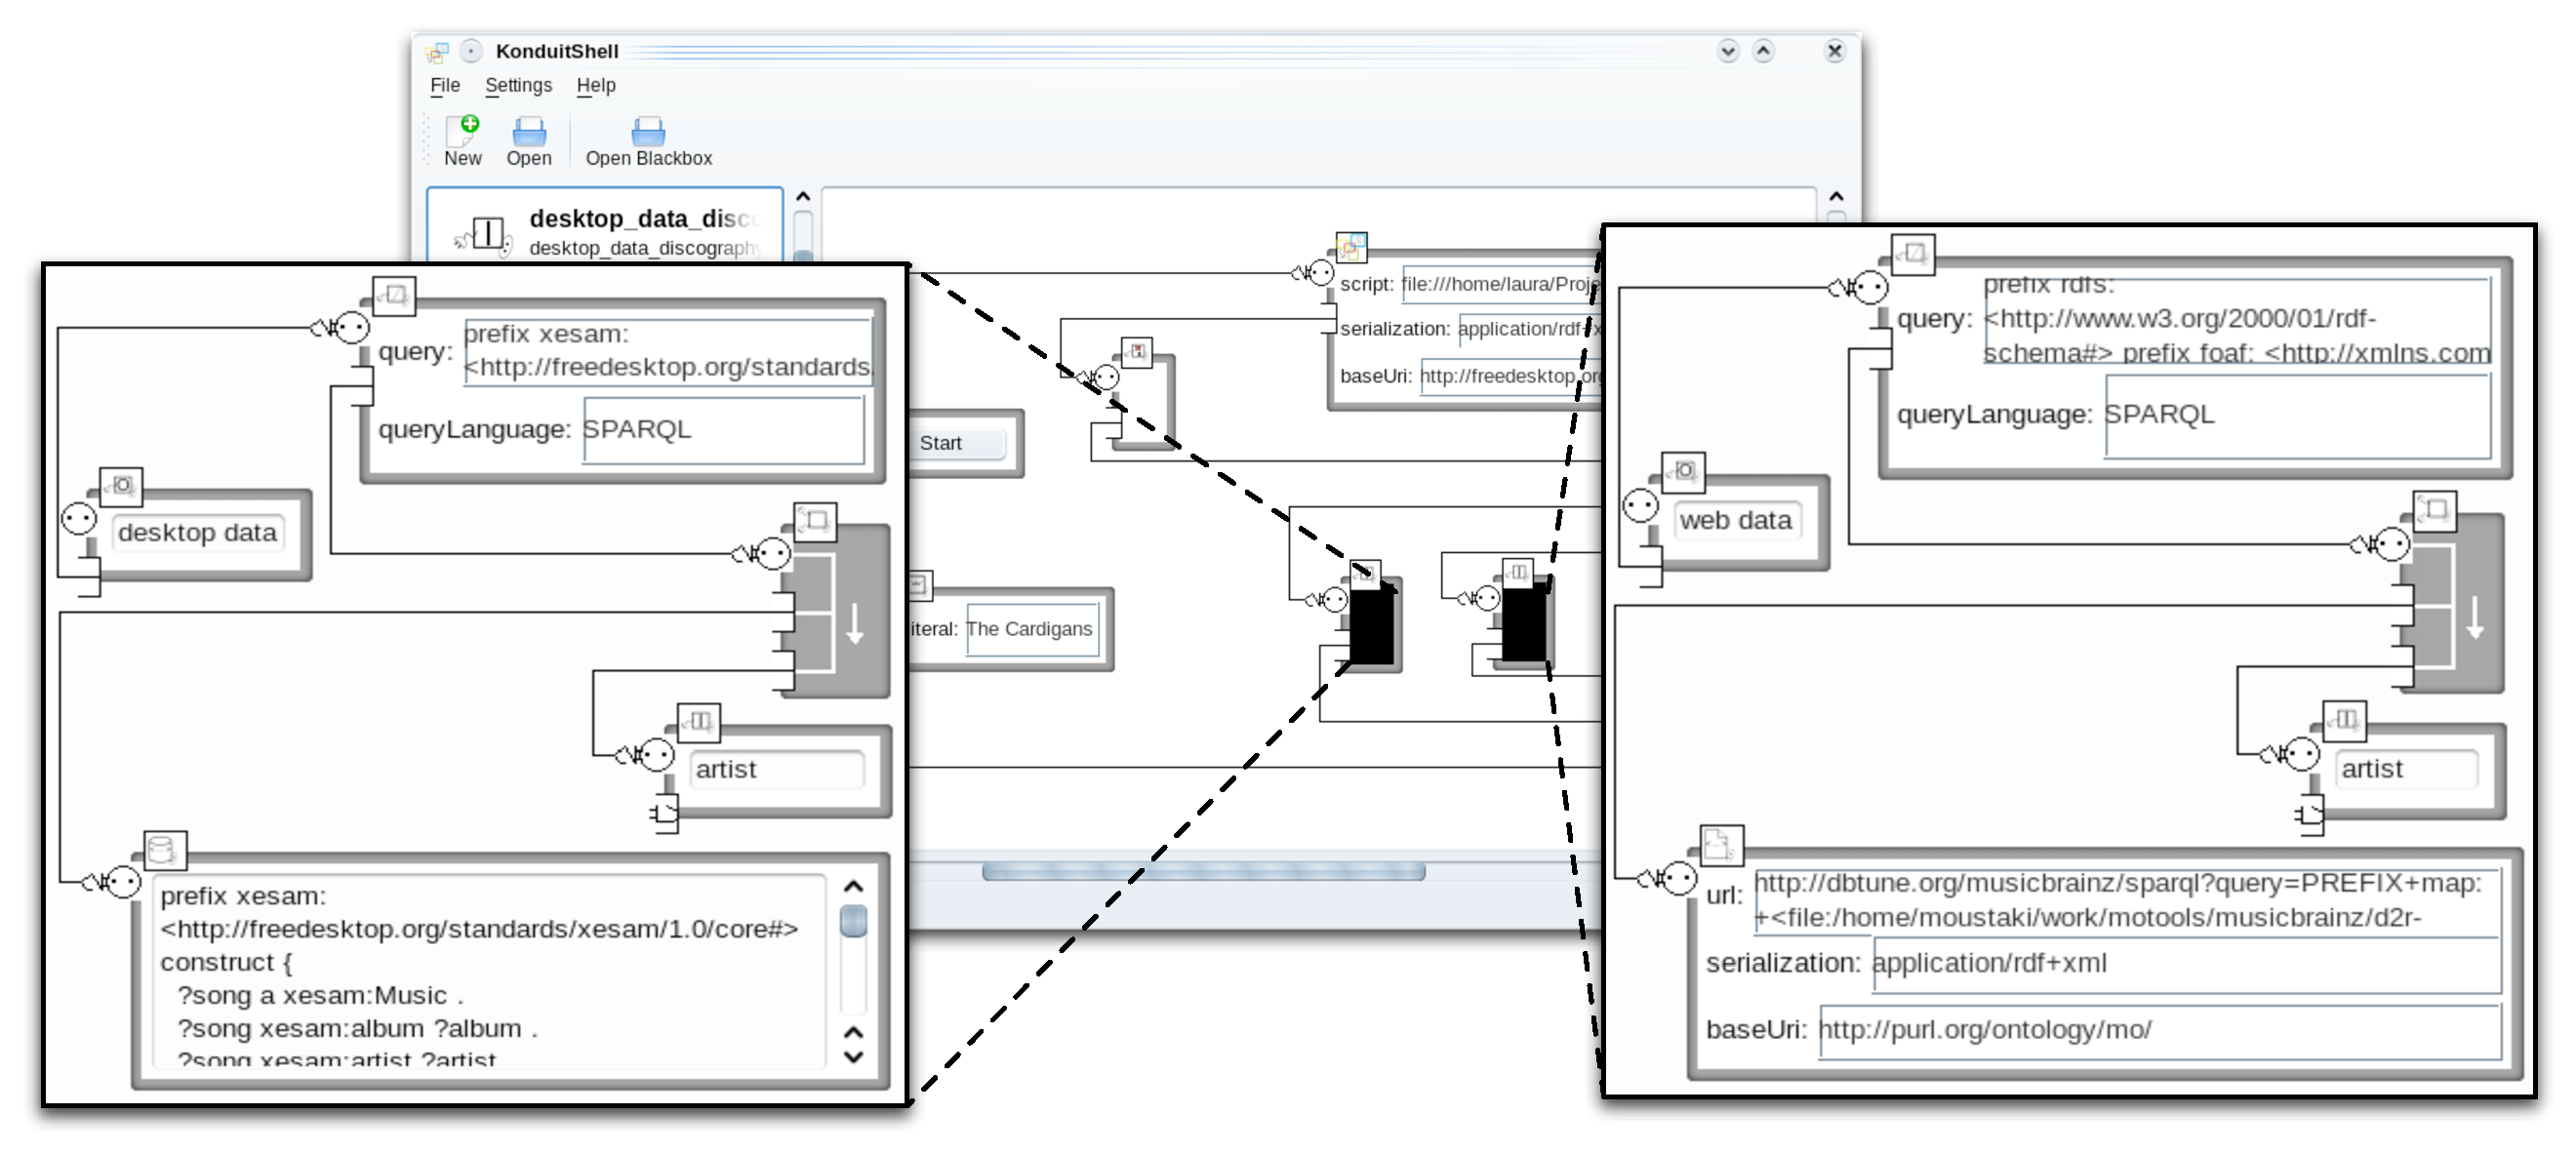
\includegraphics[width=1.0\linewidth]{chapters/core/img/discography}
 \caption{The entire discography generator workflow.}
 \label{fig:discography_generator}
\end{figure}

\cite{Dragan2009b} describes in more detail the different types of sources, sinks, and ordinary component types, as well as the blackbox mechanism. 
Some of the basic components available for Konduit require previous knowledge of writing SPARQL queries. Since the queries can influence the performance of the entire workflow, we recognise the need for a smart query editor that is suitable for naive users. \cite{Ambrus2010} describes the means for making Konduit more user friendly, by adding a smart wizard with suggestions and SPARQL autocompletion. 

